\phantomsection
\chapter[Unpacking E. coli’s Genius Exploration Algorithm]{Unpacking E. coli’s Genius Exploration Algorithm\chapsubhead{Shuanger Li and Phillip Compeau}}
\label{chapter:chemotaxis}
\renewcommand{\chaptertitle}{Unpacking E. coli’s Genius Exploration Algorithm}
\addcontentsline{cc}{chapter}{Chapter \thechapter} % Adds chapter number to table of contents


\FloatBarrier

\section{Introduction: The Lost Immortals}
\label{sec:introduction}
\phantomsection

The book \textit{What If?}, by Randall Munroe, compiles a collection of crazy scientific hypotheticals, paired with thorough discussions of what might happen if these situations occurred. Here is an example, called ``Lost Immortals''.

\begin{itquote}
If two immortal people were placed on opposite sides of an uninhabited Earth-like planet, how long would it take them to find each other? 100,000 years? 1,000,000 years?
\end{itquote}

One could imagine many ideas for how the immortals could reunite. For example, they could avoid the interiors of continents by moving to the coastlines. If they are allowed to discuss how to find each other in advance, then they could agree to meet at the planet's North Pole --- assuming that the planet lacks polar bears.

But Munroe provides a solution that is both sophisticated and elegant. His proposed approach is quoted below.

\begin{itquote}
If you have no information, walk at random, leaving a trail of stone markers, each one pointing to the next. For every day that you walk, rest for three. Periodically mark the date alongside the cairn. It doesn’t matter how you do this, as long as it’s consistent. You could chisel the number of days into a rock, or lay out rocks to plot the number.

If you come across a trail that’s newer than any you’ve seen before, start following it as fast as you can. If you lose the trail and can’t recover it, resume leaving your own trail.

You don’t have to come across the other player’s current location; you simply have to come across a location where they’ve been. You can still chase one another in circles, but as long as you move more quickly when you’re following a trail than when you’re leaving one, you’ll find each other in a matter of years or decades.

And if your partner isn’t cooperating --- perhaps they’re just sitting where they started and waiting for you --- then you’ll get to see some neat stuff.
\end{itquote}

In the previous two chapters, we have harnessed the power of randomness to answer practical questions. Munroe's approach exemplifies a \textdef{randomized algorithm}{random algorithm}{a method that uses randomness to solve a problem}, or a method that uses randomness to solve a problem.

In fact, Munroe's randomized algorithm for Lost Immortals is inspired by nature; he calls his approach ``be an ant'' because it mimics how ants explore their environment for resources. In this chapter, we will see that this algorithm is also similar to the method of exploration undertaken by a much smaller organism: our old friend \textit{E. coli}.

Like other prokaryotes, \textit{E. coli} is tiny, with a rod-shaped body that is 2 µm long and 0.25 to 1 µm wide. In exploring a vast world with sparse resources, \textit{E. coli} finds itself in a situation comparable to the Munroe's immortals.

%The video below shows a collection of \textit{E. coli} surrounding a sugar crystal. Think of this video the next time you leave a slice of cake out overnight on the kitchen counter!
%
%\texttt{NEED FIGURE HERE -- TO REPLACE VIDEO}\\

The movement of organisms like \textit{E. coli} in response to a chemical stimulus is called \textdef{chemotaxis}{chemotaxis}{the movement of an organism in response to a chemical stimulus}. \textit{E. coli} and other bacteria have evolved to move toward \textdefnogloss{attractants} like glucose and electron acceptors and move away from \textdefnogloss{repellents} like Ni\textsuperscript{2+} and Co\textsuperscript{2+}. But how?

In this chapter, we will delve into chemotaxis and ask a number of questions. How does a simple organism like \textit{E. coli} sense an attractant or repellent in its environment? How does the bacterium change its internal state in response to this environment? How can we model the bacterium's response? And how does the bacterium's behavior translate into an ``algorithm'' that it uses to explore its environment?\\

\FloatBarrier
\phantomsection
\section{\textit{E. coli} Explores Its World Via a Random Walk}
\label{sec:e_coli_explores_its_world_via_a_random_walk}

\phantomsection
\subsection{Bacterial runs and tumbles}


Every \textit{E. coli} cell has between five and twelve flagella distributed on its surface that can rotate both clockwise and counter-clockwise. When all of the flagella are rotating counter-clockwise, they form a bundle and propel the cell forward at about 20 µm per second. This speed may seem insignificant, but it is about ten times the length of the cell per second, which is analogous to a car traveling at 160 kph. When a flagellum rotates clockwise, the flagella become uncoordinated, and the bacterium stops and rotates in place.

When we examine the bacterium's movement under a microscope, we see it alternate between periods of ``running'' in a straight line and then ``tumbling'' in place (\autoref{fig:chemotaxis_intro_runtumble}). Over time, the bacterium's \textdef{run and tumble}{run and tumble model}{an alternation between traveling in a straight line and rotating in place, which models bacteria exploring their environment} exploration amounts to a \textit{random walk} through its environment, similar to the exploration approach used by the lost immortals.\\

\begin{figure}[h]
\centering
\mySfFamily
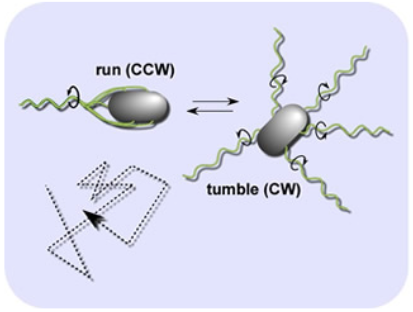
\includegraphics[width = 0.6\textwidth]{../images/chemotaxis_intro_runtumble.png}
\caption{The run and tumble mechanism of bacterial movement produces a random walk.}
\label{fig:chemotaxis_intro_runtumble}
\end{figure}

\FloatBarrier
\phantomsection
\subsection{Tumbling frequency is constant across species}

Bacteria are amazingly diverse. They have evolved for over three billion years to thrive in practically every environment on the planet, including hazardous human-made environments. They manufacture compounds such as antibiotics that larger organisms like ourselves cannot make. Some eukaryotes are even completely dependent upon bacteria to perform some critical task for them, from digesting their food, to camouflaging them from predators, to helping them develop organs.

And yet despite the diversity of the bacterial kingdom, variations in bacterial tumbling frequencies are relatively small. In the absence of an attractant or repellent, \textit{E. coli} stops to tumble once every 1 to 1.5 seconds, which is similar to most other bacteria.

It is as if there were some invisible force compelling all of these bacteria to tumble with the same frequency. Recalling Dobzhansky's quotation from \autoref{chapter:motifs} that ``nothing in biology makes sense except in the light of evolution'', we wonder how and why evolution might hold tumbling frequency constant across species.

This question is a fundamental one, and we will return to it at the close of this chapter after we have learned more about the biochemical basis of chemotaxis and how a bacterium can adjust its behavior in response to a chemical substance. In the process, we will see that despite bacteria being simple organisms, the mechanism they use to implement chemotaxis is far more sophisticated than we might expect.\\

\begin{qbox}[%
Say that a bacterium travels 20 µm per second, and every second it chooses a random direction in which to travel.  After an hour, approximately how far will it have traveled on average? What if we allow the bacterium to travel for a week? (Hint: recall the Random Walk Theorem from \autoref{chapter:turing}.)
]\end{qbox}


\FloatBarrier
\phantomsection
\section{Signaling and Ligand-Receptor Dynamics}
\label{sec:signal}

\phantomsection
\subsection{Cells detect and transduce signals via receptor proteins}

Chemotaxis is one example of many ways in which a cell must perceive a change in its environment and react accordingly. This response is governed by a process called \textdef{signal transduction}{signal transduction}{the intracellular transmission of an external stimulus in order to effect a response}, in which a cell identifies a stimulus outside the cell and then transmits this stimulus into the cell in order to effect a response. When a certain molecule's extracellular concentration increases, \textdef{receptor proteins}{receptor protein}{a protein on the surface of the cell that binds to molecules in order to detect changes in their extracellular concentration} on the outside of the cell have more frequent binding with these molecules and are therefore able to detect changes in molecular concentration. This ``signal is then ``transduced'' via a series of internal chemical processes.

For example, transcription factors, which we discussed in \autoref{chapter:motifs}, are involved in a signal transduction process. When some extracellular molecule is detected, a cascade begins that eventually changes a transcription factor into an active state, so that it is ready to activate or repress the genes that it regulates.

In the case of chemotaxis, \textit{E. coli} has receptor proteins that detect attractants such as glucose by binding to and forming a complex with these attractant \textdef{ligands}{ligand}{a substance that forms a complex with a biological molecule such as a receptor protein}. The bacterium also contains receptors to detect repellents, but we will focus on modeling the binding of a single type of receptor to a single type of attractant ligand. Later in the chapter, we will enter the cell and model the cascade of reactions after this binding has occurred, as shown in \autoref{fig:chemotaxis_signal}, which cause a change in the rotation of one or more flagella.

\begin{figure}[h]
\centering
\mySfFamily
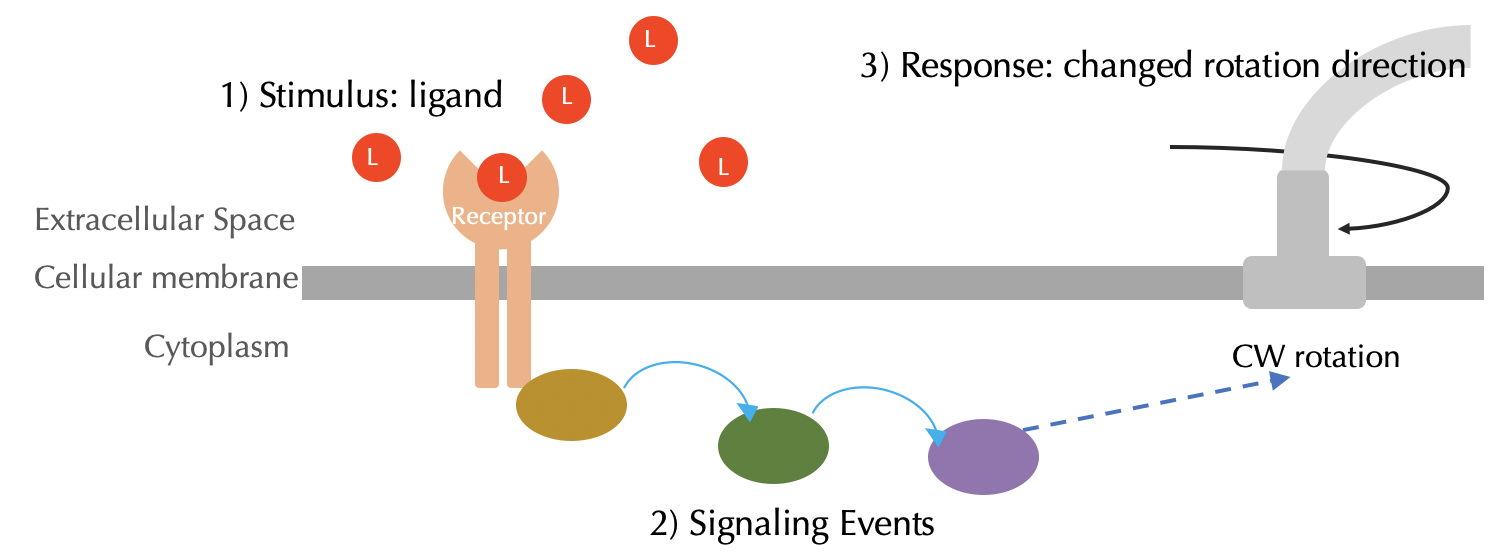
\includegraphics[width = 0.85\textwidth]{../images/chemotaxis_signal.png}
\caption{An overview of the signaling pathway of chemotaxis. The red circles labeled \textit{L} represent attractant ligands. When these ligands bind to receptors, a signal is transduced inside the cell via a series of enzymes, which finally influences the rotation direction of a flagellum.}
\label{fig:chemotaxis_signal}
\end{figure}

\FloatBarrier
\nopagebreak
\phantomsection
\subsection{Ligand-receptor dynamics correspond to a reversible reaction}

The chemical reactions that we have considered earlier in this book are \textdef{irreversible}{irreversible reaction}{a chemical reaction that only proceeds in one direction}, meaning they can only proceed in one direction. For example, in \autoref{chapter:turing}'s reaction-diffusion model, we modeled the reaction $A + 2B \rightarrow 3B$, but we did not consider the reverse reaction $3B \rightarrow A + 2B$.

To model ligand-receptor dynamics, we will use a \textdef{reversible reaction}{reversible reaction}{a chemical reaction that proceeds continuously in both directions (at possibly different rates)} that proceeds continuously in both directions at possibly different rates. If a ligand collides with a receptor, then there is some probability that the two molecules will bind into a complex. But at the same time, in any unit of time, there is also some probability that a bound receptor-ligand complex will \textdefnogloss{dissociate} into two separate molecules. In a future chapter, we will discuss the biochemical details underlying what makes two molecules more or less likely to bind, but for now, we assert that the more suited a receptor is to a ligand, the higher the binding rate and the lower the dissociation rate.\\

\begin{note}[%
Why should ligand-receptor binding be reversible? If complexes did not dissociate, then a brief increase in ligand concentration would be detected indefinitely by the surface receptors. Without releasing the bound ligands, the cell would need to manufacture more receptors, which are complicated molecules.
]\end{note}

We denote the ligand molecule by $L$, the receptor molecule by $T$, and the bound complex as $LT$. The reversible reaction is $L + T \longleftrightarrow LT$ and consists of two reactions. The \textdefnogloss{forward reaction} is $L + T \rightarrow LT$, which takes place at some rate $k_\text{bind}$, and the \textdefnogloss{reverse reaction} is $LT \rightarrow L + T$, which takes place at some rate $k_\text{dissociate}$.

If we start with a free floating supply of $L$ and $T$ molecules, then $LT$ complexes will initially be formed quickly at the expense of the free-floating $L$ and $T$ molecules. The reverse reaction will not occur because of the lack of $LT$ complexes. However, as the concentration of $LT$ grows and the concentrations of $L$ and $T$ decrease, the rate of increase in $LT$ will slow. Eventually, the number of $T$ complexes being formed by the forward reaction will balance the number of $LT$ complexes being split apart by the reverse reaction. At this point, the concentration of all particles reaches equilibrium.

\FloatBarrier
\phantomsection
\subsection{Calculation of equilibrium in a reversible ligand-receptor reaction}

For a single reversible reaction, if we know the rates of both the forward and reverse reactions, then we can calculate the steady state concentrations of $L$, $T$, and $LT$ by hand.  Suppose that we begin with initial concentrations of $L$ and $T$ that are represented by $l_0$ and $t_0$, respectively. Let $[L]$, $[T]$, and $[LT]$ denote the concentrations of the three molecule types. And assume that the reaction rate constants $k_\text{bind}$ and $k_\text{dissociate}$ are fixed.

When the steady state concentration of $LT$ occurs, the rate of production of $LT$ is equal to the rate of its dissociation; in other words, we know that

\begin{center}
$k_\text{bind} \cdot [L] \cdot [T] = k_\text{dissociate} \cdot [LT] $\,.

\end{center}

We also know that by the law of conservation of mass, the concentrations of $L$ and $T$ molecules are always constant across the system and are equal to their initial concentrations. That is, at any time point,

\begin{center}
$[L] + [LT] = l_0$
\end{center}

\noindent and

\begin{center}
$[T] + [LT] = t_0 $\,.
\end{center}

\noindent Solving these equations for $[L]$ and $[T]$ yields the following two equations:
\begin{align*}
[L] & = l_0 - [LT]\\
[T] & = t_0 - [LT]\,.
\end{align*}

We will now substitute the expressions on the right for $[L]$ and $[T]$ into our original steady state equation:

\begin{center}
$k_\text{bind} \cdot (l_0 - [LT]) \cdot (t_0 - [LT]) = k_\text{dissociate} \cdot [LT]$\,.
\end{center}

\noindent Expanding the left side of this equation gives

\begin{center}
$k_\text{bind} \cdot [LT]^2 - (k_\text{bind} \cdot l_0 + k_\text{bind} \cdot t_0) \cdot [LT]  = k_\text{dissociate} [LT] + k_\text{bind} \cdot l_0 \cdot t_0$\,.
\end{center}

\noindent Finally, we subtract the right side of this equation from both sides to give

\begin{center}
$k_\text{bind} \cdot [LT]^2 - (k_\text{bind} \cdot l_0 + k_\text{bind} \cdot t_0 + k_\text{dissociate}) \cdot [LT] + k_\text{bind} \cdot l_0 \cdot t_0 = 0$\,.
\end{center}

\noindent This equation may look daunting, but most of its components are constants. In fact, the only unknown is $[LT]$, which makes this a quadratic equation, with $[LT]$ as the variable.

In general, a quadratic equation has the form $a \cdot x^2 + b \cdot x + c = 0$ for constants $a$, $b$, and $c$ and a single variable $x$. In our case, $x$ = $[LT]$, and the constants are $a = k_\text{bind}$, $b = - (k_\text{bind} \cdot l_0 + k_\text{bind} \cdot t_0 + k_\text{dissociate})$, and $c = k_\text{bind} \cdot l_0 \cdot t_0$. The quadratic formula --- which you may have thought you would never use again --- tells us that the equation $a \cdot x^2 + b \cdot x + c = 0$  has solutions for $x$ given by

\begin{center}
$x = \dfrac{-b \pm \sqrt{b^2 - 4 \cdot a \cdot c}}{2 \cdot a}$\,.
\end{center}

\fudgespace

\begin{qbox}[%
Use the quadratic formula to find the steady state concentration of $LT$. How can we use this solution to find the steady state concentrations of $L$ and $T$ as well?
]\end{qbox}

Now that we have reduced the computation of the steady state concentration of $LT$ to the solution of a quadratic equation, let's compute this steady state concentration for a sample collection of parameters. We will then change the parameters and see how the steady state concentration changes.

Say that we are given the following parameter values (the units of these parameters are not important for this toy example):
\begin{align*}
k_\text{bind} & = 2\,;\\
k_\text{dissociate} & = 5\,;\\
l_0 & = 50\,;\\
t_0 & = 50\,.
\end{align*}

%\begin{itemize}
% \item $k_\text{bind}= 2$;
% \item $k_\text{dissociate} = 5$;
% \item $l_0 = 50$;
% \item $t_0 = 50$.
%\end{itemize}

\noindent Substituting these values into the quadratic equation, we obtain
\begin{align*}
a & = k_\text{bind} = 2\,;\\
b & = - (k_\text{bind} \cdot l_0 + k_\text{bind} \cdot t_0 + k_\text{dissociate}) = -205\,;\\
c & = k_\text{bind} \cdot l_0 \cdot t_0 = 5000\,.
\end{align*}

\noindent That is, we are solving the equation $2 \cdot [LT]^2 - 205 \cdot [LT] + 5000 = 0$. Using the quadratic formula to solve for $[LT]$ gives

\begin{center}
$[LT] = \dfrac{205 \pm \sqrt{205^2 - 4 \cdot 2 \cdot 5000}}{2 \cdot 2} = 51.25 \pm 11.25$\,.
\end{center}

It would seem that this equation has \textit{two} solutions: $51.25 + 11.25 = 62.5$ and $51.25 - 11.25 = 40$. However, because $l_0$ and $t_0$, the respective initial concentrations of $L$ and $T$, are both equal to 50, the steady state concentration of $LT$ cannot be 62.5; instead, it must be 40.

Now that we know the steady state concentration of $LT$, we can recover the values of $[L]$ and $[T]$ too:
\begin{align*}
[L] & = l_0 - [LT] = 10\,;\\
[T] & = t_0 - [LT] = 10\,.
\end{align*}

What if the forward reaction were slower (i.e., $k_\text{bind}$ was lower)? We would imagine that the equilibrium concentration of $[LT]$ would decrease. For example, if we halve $k_\text{bind}$, then we obtain the following adjusted parameter values:
\begin{align*}
a & = k_\text{bind} = 1\,;\\
b & = - (k_\text{bind} \cdot l_0 + k_\text{bind} \cdot t_0 + k_\text{dissociate}) = -105\,;\\
c & = k_\text{bind} \cdot l_0 \cdot t_0 = 2500\,.
\end{align*}

\noindent In this case, if we solve the quadratic equation for $[LT]$, then we obtain

\begin{center}
$[LT] = \dfrac{105 \pm \sqrt{105^2 - 4 \cdot 1 \cdot 2500}}{2 \cdot 1} = 52.5 \pm 16.008$\,.
\end{center}

\noindent The only reasonable solution here is $52.5-16.008 = 36.492$; the steady state concentration has decreased as anticipated.\\

\begin{qbox}[%
What do you think will happen to the steady state concentration of $L$ if its initial concentration ($l_0$) increases or decreases? What if the dissociation rate ($k_\text{dissociate}$) increases or decreases?  Confirm your prediction by changing the parameters above and solving the quadratic formula for the concentration of $L$.
]\end{qbox}

\FloatBarrier
\phantomsection
\subsection{Where are the units?}

We have conspicuously not provided any units in the calculations above for the sake of simplicity, and so we will pause to explain what these units are. The concentration of a particle (whether it is $[L]$, $[T]$, or $[LT]$) is measured in $\text{molecules}/\text{µm}^3$, the number of molecules per unit volume. But what about the binding and dissociation rates?

When we multiply the binding rate $k_\text{bind}$ by the concentrations $[L]$ and $[T]$, the resulting unit should be in $\text{molecules}/\text{µm}^3$ per second, which corresponds to the rate at which the concentration of $LT$ complexes is increasing. If we let \textvar{x} denote the unknown units of $k_\text{bind}$, then we should have that

\begin{center}
$x \cdot (\text{molecules}/\text{µm}^3) \cdot (\text{molecules}/\text{µm}^3) = (\text{molecules}/\text{µm}^3) \cdot s^{-1}$\,,
\end{center}

\noindent and solving for \textvar{x} gives us that

\begin{center}
$x = (\text{µm}^3/\text{molecule}) \cdot s^{-1}$\,.
\end{center}

\fudgespace

\begin{qbox}[%
Use a similar argument to show that the units of the dissociation rate $k_\text{dissociate}$ should be $s^{-1}$.
]\end{qbox}

\FloatBarrier
\phantomsection
\subsection{Steady state ligand-receptor concentrations for an experimentally verified example}

Let's use experimentally verified binding and dissociation rates to identify steady state concentrations. The experimentally verified binding rate is $k_\text{bind} = 0.0146~(\text{µm}^3/\text{molecule}) \cdot s^{-1}$, and the dissociation rate constant is $k_\text{dissociate} = 35s^{-1}$\,. We will model an \textit{E. coli} cell with 7,000 receptor molecules in an environment containing 10,000 ligand molecules. Using these values, we obtain the following constants $a$, $b$, and $c$ in the quadratic equation:
\begin{align*}
a & = k_\text{bind} = 0.0146\,;\\
b & = - (k_\text{bind} \cdot l_0 + k_\text{bind} \cdot t_0 + k_\text{dissociate}) = -283.2\,;\\
c & = k_\text{bind} \cdot l_0 \cdot t_0 = 1022000\,.
\end{align*}

When we solve for $[LT]$ in the quadratic equation, we obtain $[LT]$ equal to 4,793 $\text{molecules}/\text{µm}^3$. Now that we have this value along with $l_0$ and $t_0$, we can solve for $[L]$ and $[T]$ as well:
\begin{align*}
[L] & = l_0 - [LT] = \text{5,207 molecules}/\text{µm}^3\,;\\
[T] & = t_0 - [LT] = \text{2,207 molecules}/\text{µm}^3\,.
\end{align*}

We can therefore determine the steady state concentration for a \textit{single} reversible reaction. However, if we want to model real cellular processes, we will have \textit{many} reactions for a variety of different particles. We will see that it quickly becomes infeasible to solve all of the resulting equations exactly. Instead, we need a method of simulating many reactions in parallel without incurring the significant computational overhead that would be required to keep track of every individual particle.\\

\FloatBarrier
\phantomsection

\section{Stochastic Simulation of Chemical Reactions}
\label{sec:stochastic_simulation_of_chemical_reactions}
\phantomsection
\subsection{Verifying a theoretical steady state concentration via stochastic simulation}

In \autoref{chapter:motifs}, we saw that we could avoid tracking the positions of individual particles if we assume that the particles are \textit{well-mixed}, i.e., uniformly distributed throughout their environment. We will apply this assumption in our current work as well, in part because the \textit{E. coli} cell is so small. As a proof of concept, let us first see if a well-mixed simulation replicates the steady state concentrations of particles that we found in \autoref{sec:signal}.

Even though we can calculate steady state concentrations by hand, a particle-free simulation will be useful for two reasons. First, this simulation will give us snapshots of the concentrations of particles in the system over multiple time points and allow us to see how quickly the concentrations reach equilibrium. Second, we will soon expand our model of chemotaxis to have many particles and reactions that depend on each other, and direct mathematical analysis of the system like what we have done in the previous section will become impossible.

The difficulty at hand is comparable to the famed ``\textit{n}-body problem'' in physics. Predicting the motions of two celestial objects interacting due to gravity can be done exactly, but there is no known such solution once we add more bodies to the system.

Our particle-free model will apply an approach called \textdef{Gillespie's stochastic simulation algorithm}{Gillespie's stochastic simulation algorithm (SSA)}{an algorithm that simulates a well-mixed environment of particles by apply repeated sampling from an exponential distribution to determine time between reactions}, which is often called the \textbf{Gillespie algorithm} or just \textbf{SSA} for short. Before we explain how this algorithm works, we take a short detour to provide some needed probabilistic context.

\FloatBarrier
\phantomsection
\subsection{The Poisson and exponential distributions}

Say that you own a store and have noticed that on average, there are $\lambda$ customers entering your store in a single hour. Let \textvar{X} denote the number of customers that enter the store in the next hour; \textvar{X} is an example of a \textdef{random variable}{random variable}{a variable whose values may change based on random chance} because it may change depending on random chance. If we assume that customers are independent actors arriving at a constant rate, then \textvar{X} follows a \textdef{Poisson distribution}{Poisson distribution}{a distribution representing the probability of a number of events occurring in a fixed time interval if these events occur independently at a fixed rate}. It can be shown that for a Poisson distribution, the probability that exactly $n$ customers arrive in the next hour is

\begin{center}
$\mathrm{Pr}(X = n) = \dfrac{\lambda^n e^{-\lambda}}{n!}$\,,
\end{center}

\noindent where $e$ is the mathematical constant known as Euler's number and is equal to 2.7182818284\ldots\\

\begin{note}[
A derivation of this formula is beyond the scope of our work here, but if you are interested in one, please check out \href{https://medium.com/@andrew.chamberlain/deriving-the-poisson-distribution-from-the-binomial-distribution-840cc1668239} by Andrew Chamberlain.
]\end{note}

Furthermore, the probability of observing exactly $n$ customers in $t$ hours where $t$ is an arbitrary positive number is

\begin{center}
$\dfrac{(\lambda t)^n e^{-\lambda t}}{n!}$\,.
\end{center}

We can also ask how long we will typically have to wait for the next customer to arrive. Specifically, what are the chances that this customer will arrive after $t$ hours? If we let \textvar{T} be the random variable corresponding to the wait time on the next customer, then the probability of \textvar{T} being at least $t$ is the probability of seeing zero customers in $t$ hours:

\begin{center}
$\mathrm{Pr}(T > t) = \mathrm{Pr}(X = 0) = \dfrac{(\lambda t)^0 e^{-\lambda t}}{0!} = e^{-\lambda t}$\,.
\end{center}

In other words, the probability $\mathrm{Pr}(T > t)$ decays exponentially over time as \textvar{t} increases. For this reason, the random variable \textvar{T} is said to follow an \textdef{exponential distribution}{exponential distribution}{a distribution representing the ``wait time'' between successive events in a Poisson distribution}. It can be shown that the expected value of the exponential distribution (i.e., the average amount of time we will need to wait for the next event to occur) is $1/\lambda$.\\

\begin{qbox}[%
What is the probability $\mathrm{Pr}(T < t)$?
]\end{qbox}


\FloatBarrier
\phantomsection
\subsection{The Gillespie algorithm}

The engine of the Gillespie algorithm runs on a single question: given a well-mixed environment of particles and a reaction involving those particles taking place at some average rate, how long should we expect to wait before this reaction occurs somewhere in the environment?

This is the same question we asked in the previous section; we have simply replaced customers entering a store with instances of a chemical reaction. The average number $\lambda$ of occurrences of the reaction in a unit time period is the rate at which the reaction occurs. Therefore, an exponential distribution with average wait time $1/\lambda$ can be used to model the time between instances of the reaction.

Next, say that we have two reactions proceeding independently of each other and occurring at average rates $\lambda_1$ and $\lambda_2$. Then the average rate of the two reactions together is $\lambda_1 + \lambda_2$, which is also a Poisson distribution. Therefore, the wait time for either of the two reactions is exponentially distributed, with an average wait time equal to $1/(\lambda_1 + \lambda_2)$.

Numerical methods allow us to generate a random number simulating the wait time of an exponential distribution. By repeatedly generating these numbers, we can obtain a series of wait times between consecutive reaction occurrences.

Once a wait time is selected, we should determine to which of the two reactions it corresponds. If the rates of the two reactions are equal, then we simply choose one of the two reactions randomly with equal probability. But if the rates of these reactions are different, then we should choose one of the reactions via a probability that is \textit{weighted} in direct proportion to the rate of the reaction; that is, the larger the rate of the reaction, the more likely that this reaction corresponds to the current event. To do so, we select the first reaction with probability $\lambda_1/(\lambda_1 + \lambda_2)$ and the second reaction with probability $\lambda_2/(\lambda_1 + \lambda_2)$.\\

\begin{qbox}[%
Verify that these two probabilities sum to 1.
]\end{qbox}

As illustrated in \autoref{fig:chemotaxis_visualizessa}, we will demonstrate the Gillespie algorithm by returning to our ongoing example, in which we are modeling the forward and reverse reactions of ligand-receptor binding and dissociation. First, we choose a wait time according to an exponential distribution with mean value $1/(k_\text{bind} + k_\text{dissociate})$. The probability that the event corresponds to a binding reaction is given by

\begin{center}
$\mathrm{Pr}(L + T \rightarrow LT) = \dfrac{k_\text{bind}}{k_\text{bind} + k_\text{dissociate}}$\,,
\end{center}

\noindent and the probability that it corresponds to a dissociation reaction is

\begin{center}
$\mathrm{Pr}(L + T \rightarrow LT) = \dfrac{k_\text{dissociate}}{k_\text{bind} + k_\text{dissociate}}$\,.
\end{center}

\begin{figure}[h]
\centering
\mySfFamily
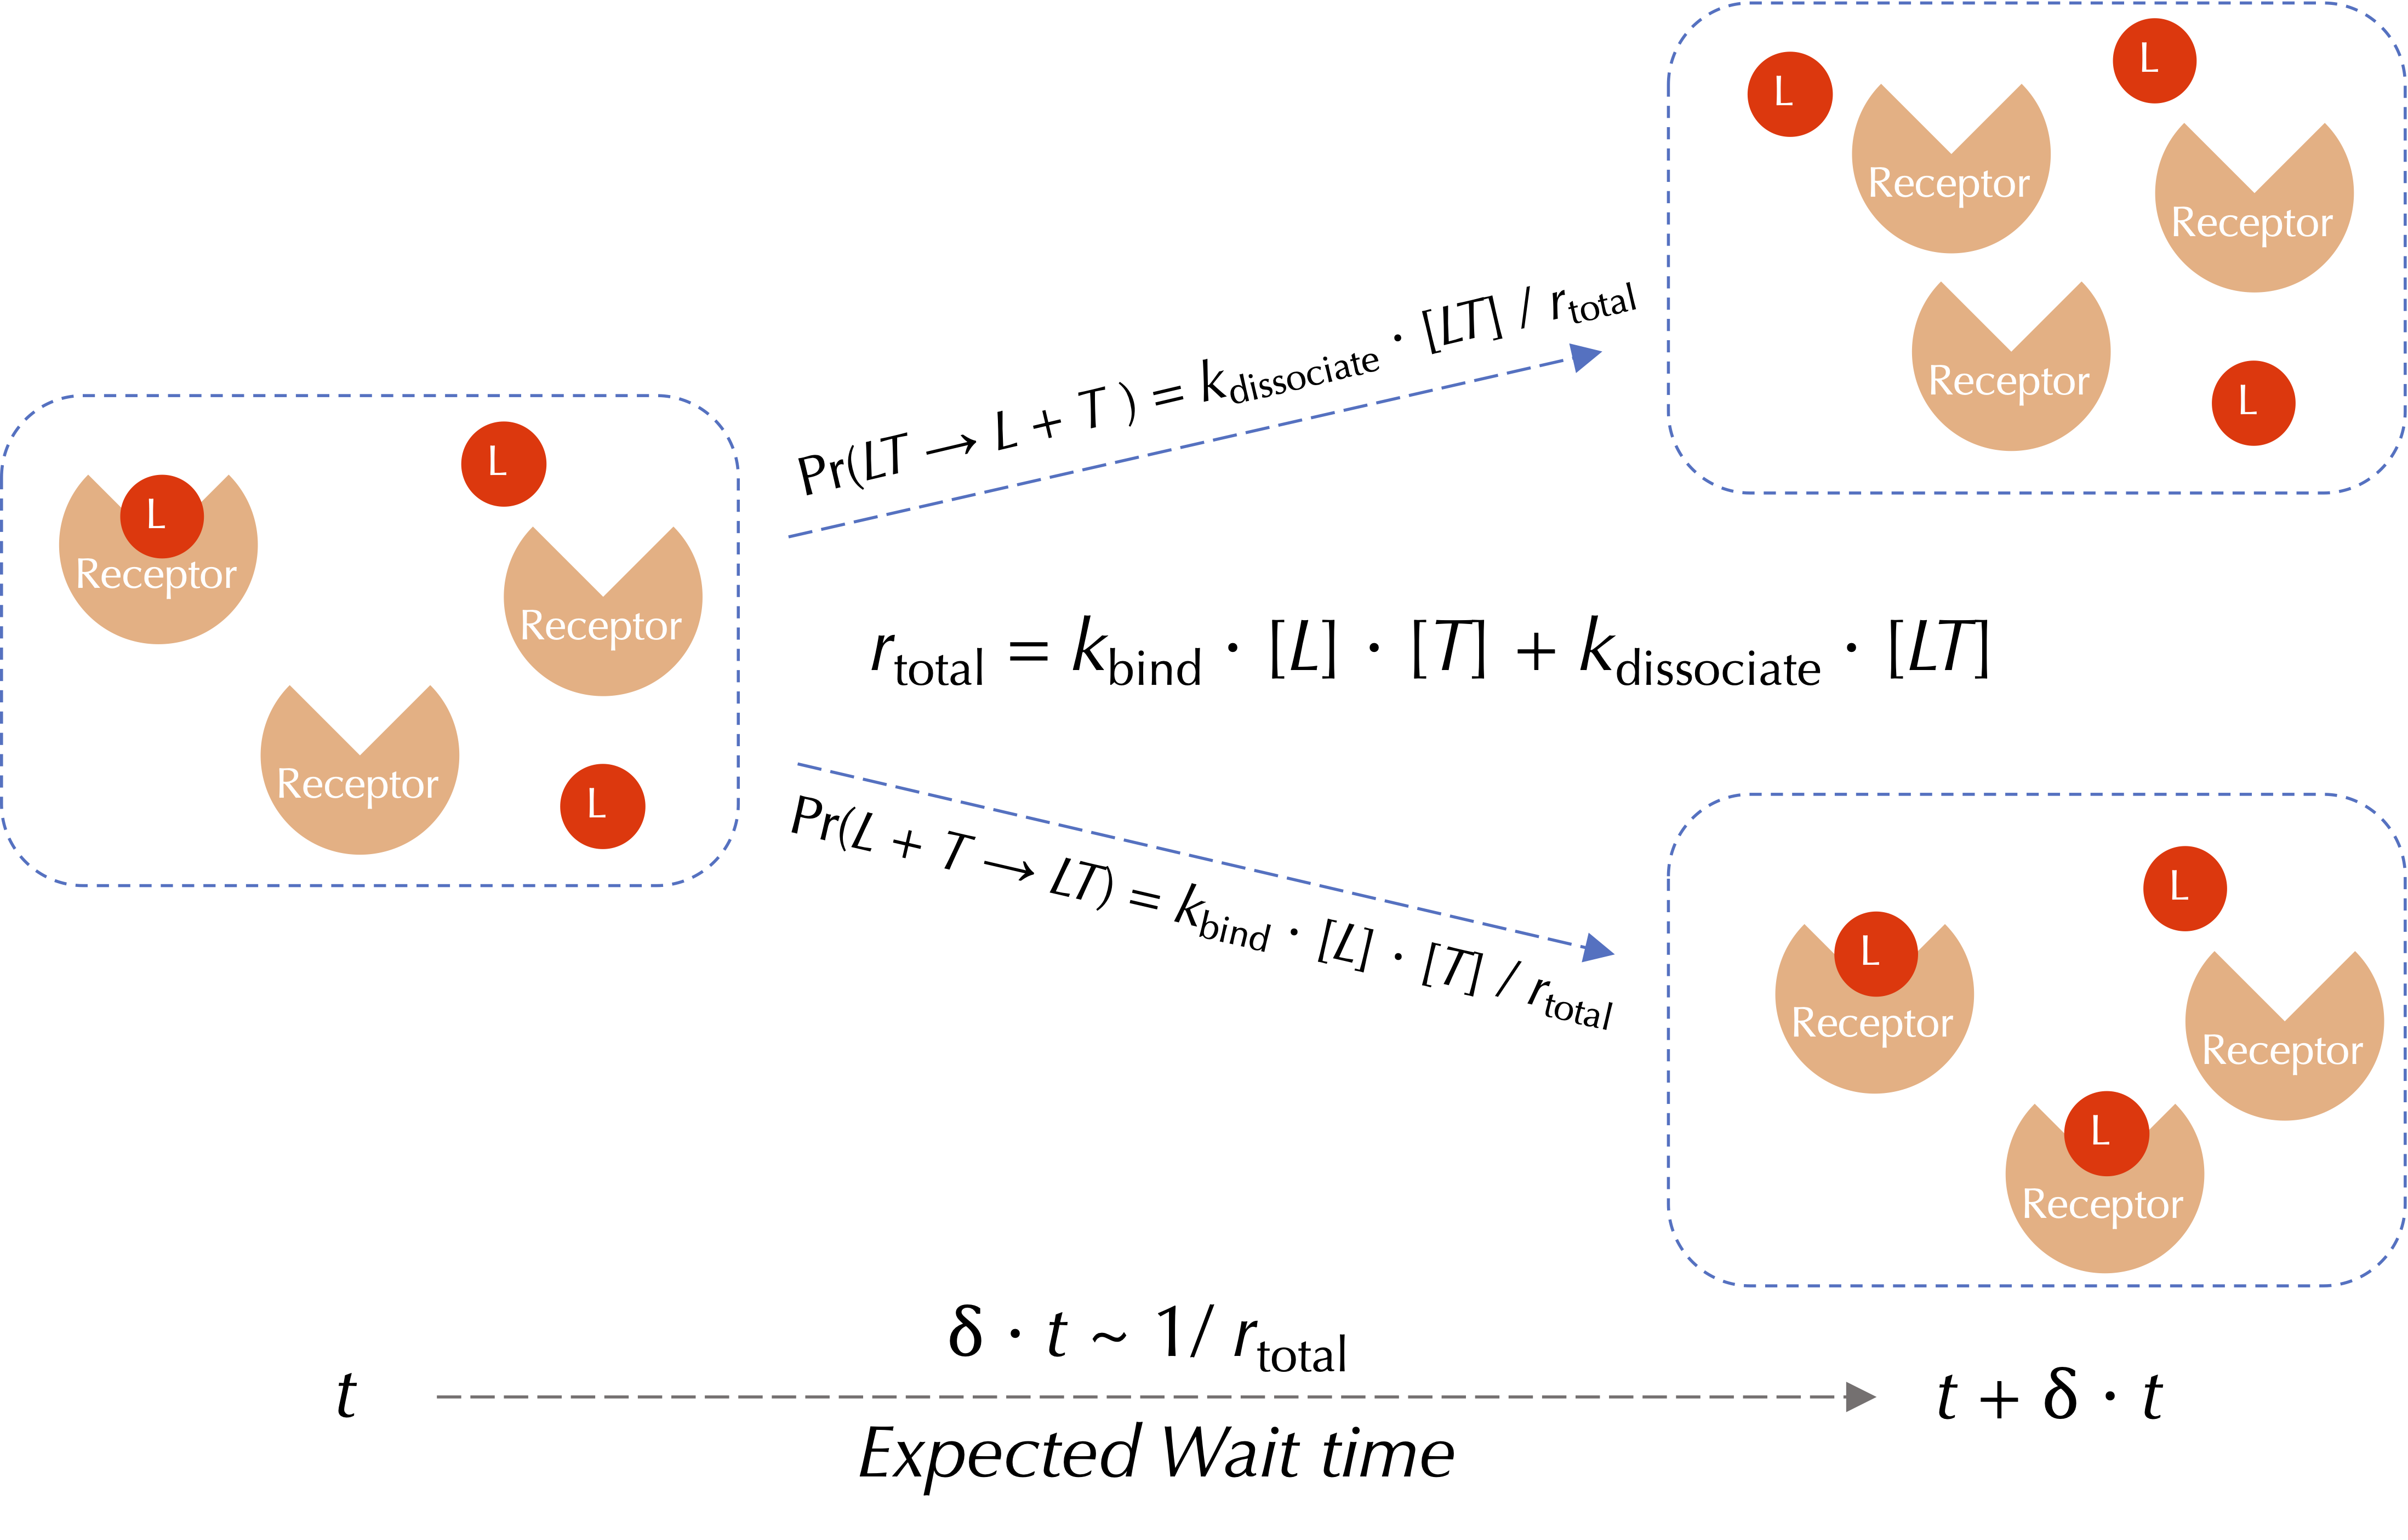
\includegraphics[width = 0.85\textwidth]{../images/chemotaxis_visualizessa.png}
\caption{A visualization of a single reaction event used by the Gillespie algorithm for ligand-receptor binding and dissociation. Red circles represent ligands (\textvar{L}), and orange wedges represent receptors (\textvar{T}). The wait time for the next reaction is drawn from an exponential distribution with mean $\text{1}/(\textvar{k}_\text{bind} + \textvar{k}_\text{dissociate})$. The probability of this event corresponding to a binding or dissociation reaction is proportional to the rate of the respective reaction.}
\label{fig:chemotaxis_visualizessa}
\end{figure}

When we generalize the Gillespie algorithm to \textvar{n} reactions occurring at rates $\lambda_1$, $\lambda_2$, \ldots, $\lambda_n$, the wait time between reactions will be exponentially distributed with average $1 / (\lambda_1 + \lambda_2 + \cdots + \lambda_n)$. Once we select the next reaction to occur, the likelihood that it is the \textvar{i}-th reaction is equal to

\begin{center}
$\lambda_i/(\lambda_1 + \lambda_2 + \cdots + \lambda_n)$\,.
\end{center}

\FloatBarrier
\phantomsection
\subsection{Specifying ligand-receptor binding with a single BioNetGen rule}

Throughout this chapter, we will employ BioNetGen (\href={http://bionetgen.org/}) to apply the Gillespie algorithm to well-mixed models of chemical reactions. We will use our ongoing example of ligand-receptor binding and dissociation to introduce the way in which BioNetGen represents molecules and reactions involving them.

We will have two molecules corresponding to the ligand and receptor $[L]$ and $[T]$ that we denote \texttt{L(t)} and \texttt{T(l)}, respectively. The \texttt{(t)} specifies that molecule \texttt{L} contains a binding site with \texttt{T}, and the \texttt{(l)} specifies a component binding to \texttt{L}. We will use these components later when specifying reactions.

BioNetGen reaction rules are written similarly to chemical equations. The left side of the rule includes the reactants, which are followed by a unidirectional or bidirectional arrow, indicating the direction of the reaction, and the right side of the rule includes the products. After the reaction, we indicate the rate constant of reaction; if the reaction is bi-directional, then we separate the forward and backward reaction rate constants with a comma.

For example, to represent the bi-directional reaction $A + B \longleftrightarrow C$ with forward rate $k_1$ and reverse rate $k_2$, we would write \texttt{A + B <-> C k1, k2}.

Our model consists of one bidirectional reaction and will have a single rule. The left side of this rule will be \texttt{L(t) + T(l)}; by specifying \texttt{L(t)} and \texttt{T(l)}, we indicate to BioNetGen that we are only interested in \textit{unbound} ligand and receptor molecules. If we had wanted to select any ligand molecule, then we would have used \texttt{L + T}.

On the right side of the rule, we will have \texttt{L(t!1).T(l!1)}, which indicates the formation of the complex. In BioNetGen, \texttt{!} indicates formation of a bond, and a unique character specifies the possible location of this bond. In our case, we use the character \texttt{1}, so that the bond is represented by \texttt{!1}. The symbol \texttt{.} is used to indicate that the two molecules are joined into a complex.

Since the reaction is bidirectional, we will use \texttt{k\_lr\_bind} and \texttt{k\_lr\_dis} to denote the rates of the forward and reverse reactions, respectively. (We will specify values for these parameters later.)

As a result, this reaction is shown below. We name our rule specifying the ligand-receptor reaction \texttt{LR}.

\begin{verbatim}
LR: L(t) + T(l) <-> L(t!1).T(l!1) k_lr_bind, k_lr_dis
\end{verbatim}

The tutorial \tutorial[https://biologicalmodeling.org/chemotaxis/tutorial\_lr] shows how to implement this rule in BioNetGen and use the Gillespie algorithm to determine the equilibrium of a reversible ligand-receptor binding reaction.


\FloatBarrier
\phantomsection
\subsection{Does the Gillespie algorithm confirm our steady state calculations?}

Earlier in this chapter, we showed an example in which a system with 10,000 free ligand molecules and 7,000 free receptor molecules produced the following steady state concentrations using the experimentally verified binding rate of $k_\text{bind} = 0.0146 (\text{µm}^3/\text{molecule}) \cdot s^{-1}$ and dissociation rate of $k_\text{dissociate} = 35s^{-1}$.
\begin{align*}
[LT] & = \text{4,793 molecules}/\text{µm}^3\\
[L] & = \text{5,207molecules}/\text{µm}^3\\
[T] & = \text{2,207 molecules}/\text{µm}^3
\end{align*}

Our BioNetGen model uses the same number of initial molecules and the same reaction rates. The system evolves via the Gillespie algorithm, and we track the concentration of free ligand molecules, ligand molecules bound to receptor molecules, and free receptor molecules over time.

\autoref{fig:chemotaxis_tutorial4_ssa} demonstrates that the Gillespie algorithm quickly converges to the same values as the ones that we obtained by hand in the last section. We are now ready to apply this algorithm to model bacterial chemotaxis, a system that will involve many different reactions.

\begin{figure}[h]
\centering
\mySfFamily
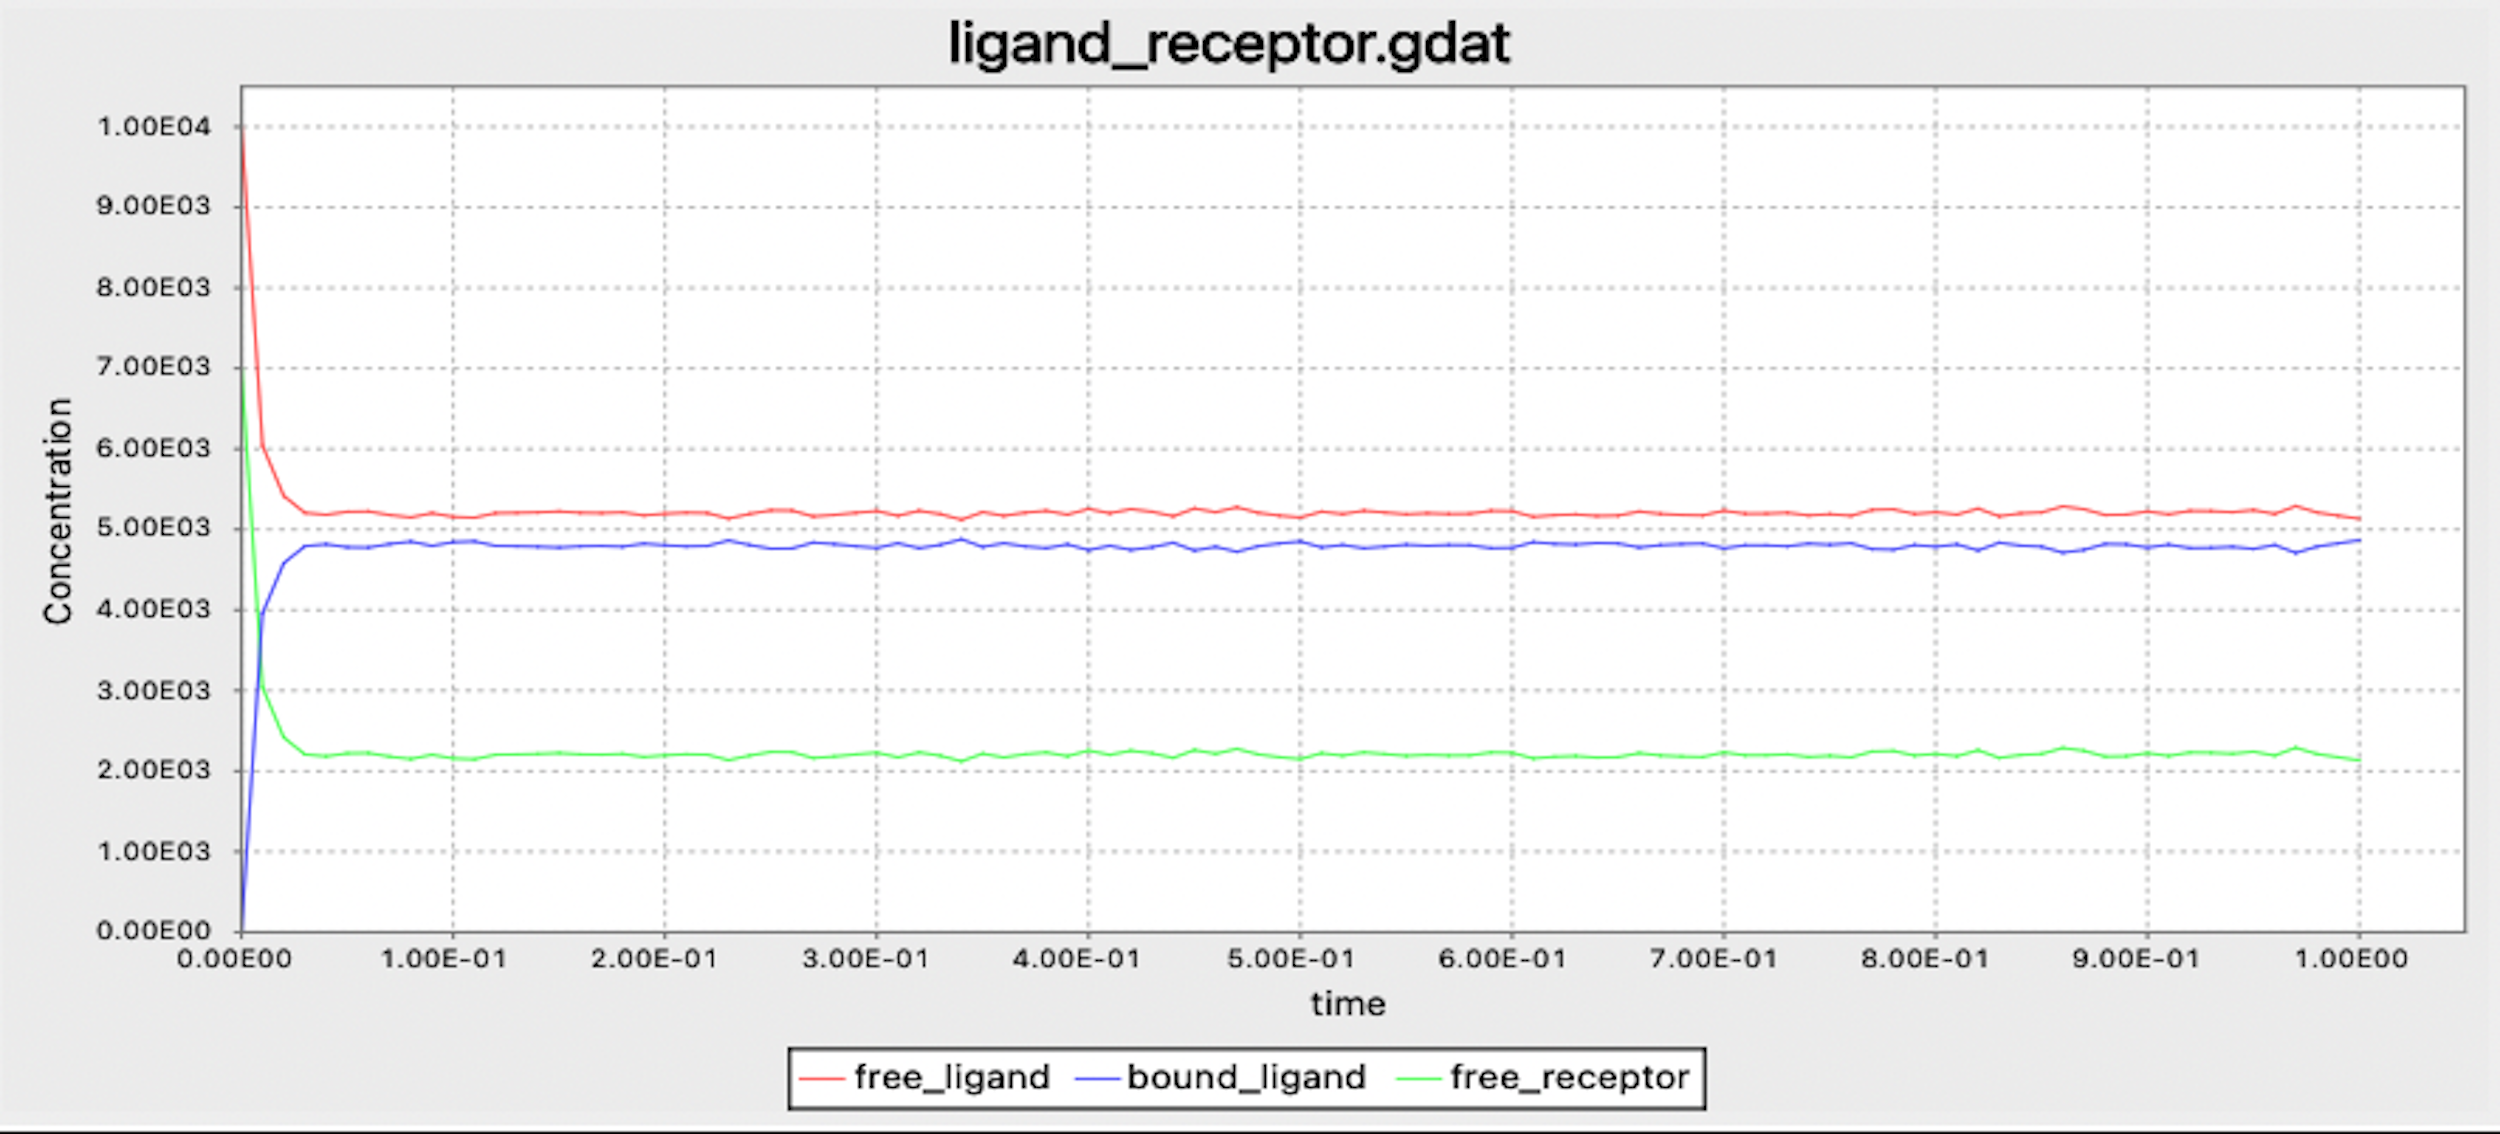
\includegraphics[width = 0.85\textwidth]{../images/chemotaxis_tutorial4_ssa.png}
\caption{A concentration plot over time for ligand-receptor dynamics via a BioNetGen simulation employing the Gillespie algorithm. Time is shown (in seconds) on the x-axis, and concentration is shown (in $\text{molecules}/\text{µm}^\text{3}$) on the y-axis. The concentrations reach a steady state at the end of the simulation that matches the concentrations identified by hand.}
\label{fig:chemotaxis_tutorial4_ssa}
\end{figure}

Yet this simple ligand-receptor model is just the beginning of our study of chemotaxis. In the next section, we will delve into the complex biochemical details of chemotaxis. Furthermore, we will see that the Gillespie algorithm for stochastic simulations will scale easily as our model of this system grows more complex.

\FloatBarrier
\phantomsection

\section{A Biochemically Accurate Model of Bacterial Chemotaxis}
\label{sec:a_biochemically_accurate_model_of_bacterial_chemotaxis}

\phantomsection
\subsection{Transducing a signal to a cell's interior}

In the previous two sections, we discussed how a cell recognizes an extracellular signal when receptor proteins on the cell's surface bind to ligands, and how to model the reversible ligand-receptor reaction using stochastic simulation via the Gillespie algorithm. We now turn to the question of how the cell conveys the extracellular signal it has detected via the process of signal transduction to the cell's interior and produces an action.

For example, if \textit{E. coli} senses an increase in the concentration of glucose, meaning that more ligand-receptor binding is taking place at the receptor that recognizes glucose, how does the bacterium \textit{E. coli} change its behavior as a result of this increased binding?

The engine of signal transduction is \textdef{phosphorylation}{phosphorylation}{a chemical reaction that attaches a phosphoryl group to an organic molecule}, a chemical reaction that attaches a phosphoryl group ($\text{PO}_3^{-}$) to an organic molecule.  Phosphoryl modifications serve as an information exchange of sorts because they activate or deactivate certain enzymes.

A phosphoryl group usually comes from one of two sources. First, the phosphoryl can be broken off of an \textdef{adenosine triphosphate (ATP)}{adenosine triphosphate (ATP)}{a molecule serving as the ``energy currency'' of the cell} molecule, the ``energy currency'' of the cell, producing \textdefnogloss{adenosine diphosphate (ADP)}. Second, the phosphoryl can be exchanged from a phosphorylated molecule that has had its phosphoryl group removed in a \textdef{dephosphorylation}{dephosphorylation}{a chemical reaction that removes a phosphoryl group from an organic molecule} reaction.

For many cellular responses, including bacterial chemotaxis, a sequence of phosphorylation and dephosphorylation events called a \textdefnogloss{phosphorylation cascade} serves to transmit information within the cell about the amount of ligand binding being detected on the cell's exterior. In this section, we discuss how this cascade of chemical reactions leads to a change in bacterial movement.

\FloatBarrier
\phantomsection
\subsection{Chemotaxis pathway}

A high-level view of the transduction pathway for chemotaxis is shown in \autoref{fig:chemotaxisphosnew}. The cell membrane contains receptors called \textdefnogloss{methyl-accepting chemotaxis proteins (MCPs)} that bridge the cellular membrane, binding both to ligand stimuli in the cell exterior and to other proteins on the inside of the cell. The pathway includes a number of additional proteins, which all start with the prefix \textit{Che} (short for ``chemotaxis'').

\begin{figure}[h]
\centering
\mySfFamily
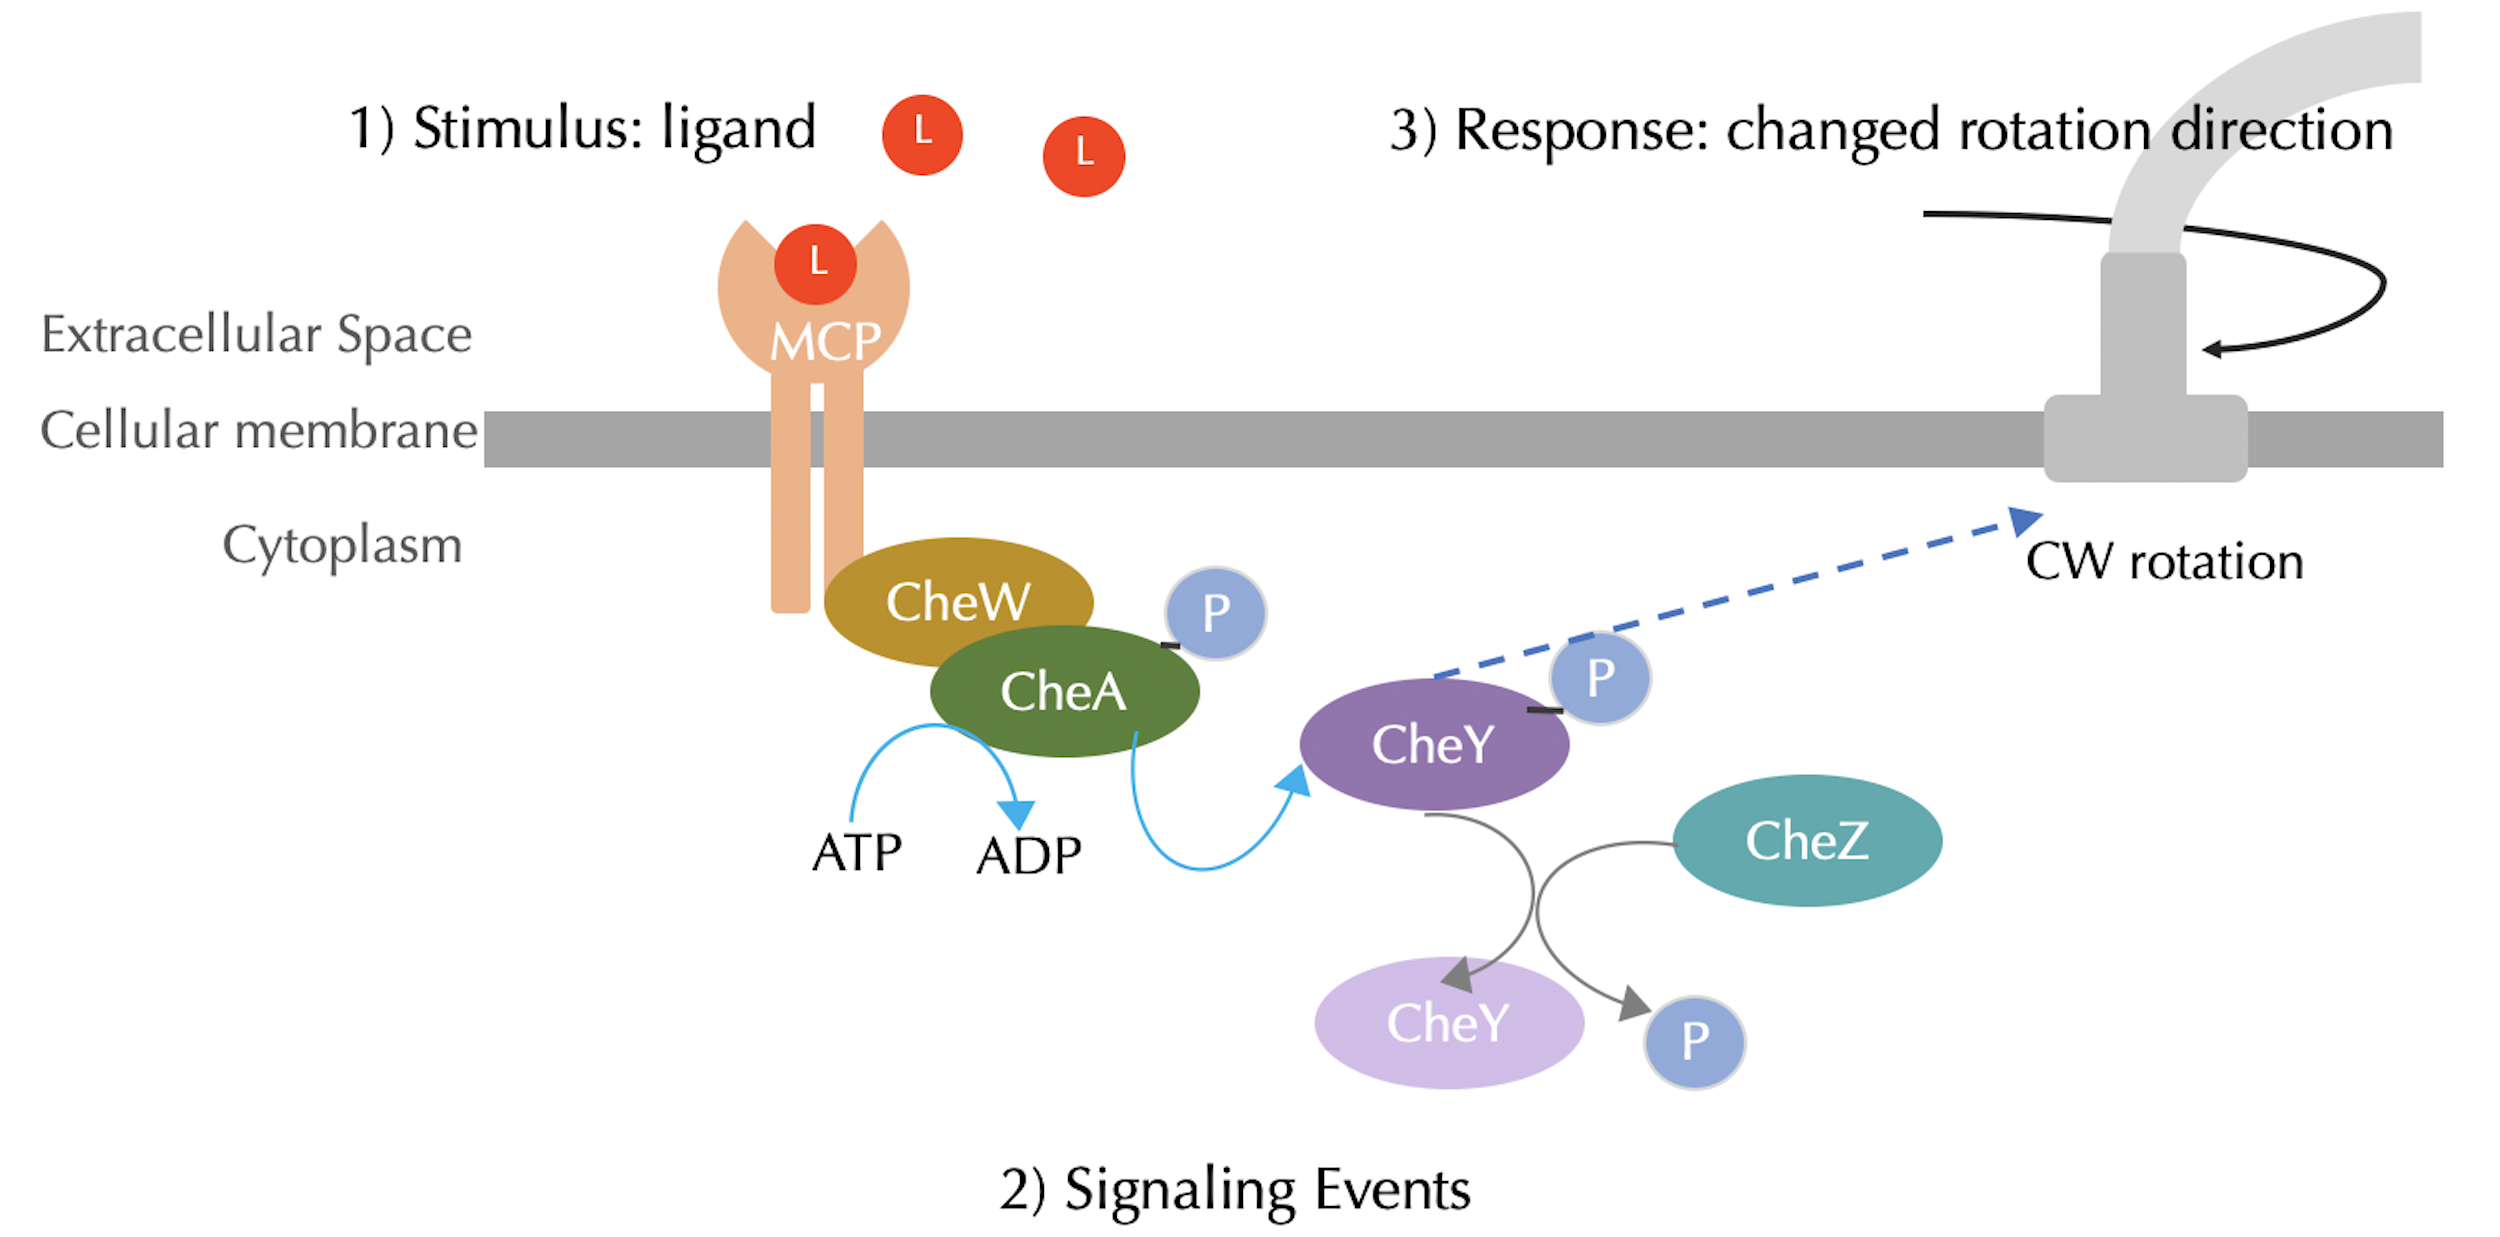
\includegraphics[width = 0.85\textwidth]{../images/chemotaxisphosnew.png}
\caption{A summary of the chemotaxis transduction pathway. A ligand binding signal is propagated through CheA and CheY phosphorylation, which leads to a response of clockwise flagellar rotation. The blue curved arrow denotes phosphorylation, the grey curved arrow denotes dephosphorylation, and the blue dashed arrow denotes a chemical interaction. Our figure is a simplified view of \href{http://chemotaxis.biology.utah.edu/Parkinson_Lab/projects/ecolichemotaxis/ecolichemotaxis.html} illustrations.}
\label{fig:chemotaxisphosnew}
\end{figure}


On the interior of the cellular membrane, MCPs form complexes with two proteins called \textbf{CheW} and \textbf{CheA}. In the absence of MCP-ligand binding, this complex is more stable, and the CheA molecule \textdef{autophosphorylates}{autophosphorylation}{the process of a molecule adding a phosphoryl group to itself}, meaning that it adds a phosphoryl group taken from ATP to \textit{itself} --- a concept that might seem mystical if you have not already followed our discussion of autoregulation in \autoref{chapter:motifs}.

Phosphorylated CheA can pass on its phosphoryl group to a molecule called \textbf{CheY}, which interacts with the flagellum in the following way. Each flagellum has a protein complex called the \textdef{flagellar motor switch}{flagellar motor switch}{a protein complex on a flagellum that is responsible for controlling the direction of flagellar rotation} that is responsible for controlling the direction of flagellar rotation. The interaction of this protein complex with phosphorylated CheY induces a change of flagellar rotation from counter\-clockwise to clockwise. As we discussed earlier in the chapter, this change in flagellar rotation causes the bacterium to tumble, which in the absence of an increase in attractant occurs every 1 to 1.5 seconds.

Yet when a ligand binds to the MCP, the MCP undergoes conformation changes, which reduce the stability of the complex with CheW and CheA. As a result, CheA is less readily able to autophosphorylate, which means that it does not phosphorylate CheY, which cannot change the flagellar rotation to clockwise, and so the bacterium is less likely to tumble.

In other words, the exchange of phosphoryl groups means that a ligand exterior to the cell can indirectly serve as an inhibitor for phosphorylated CheA as well as phosphorylated CheY. Thus, ligand binding \textit{causes} fewer flagellar interactions and in turn less tumbling of the bacterium, so that the bacterium will run for a longer stretch of time.

A critical part of the process is that if a ligand is detected, and the cell has a high concentration of CheY, then it needs to decrease the CheY concentration quickly. Otherwise, the cell will not be able to change its tumbling frequency. To this end, the cell is able to dephosphorylate CheY using an enzyme called \textbf{CheZ}.


\FloatBarrier
\phantomsection
\subsection{Adding phosphorylation events to our model of chemotaxis}


We would like to simulate the reactions driving chemotaxis signal transduction and see what happens if the bacterium ``senses an attractant'', meaning that the attractant ligand's concentration increases and leads to more receptor\-ligand binding. To do so, we will use the Gillespie algorithm.

This model will be more complicated than any we have introduced thus far. We will need to account for both bound and unbound MCP molecules, as well as phosphorylated and unphosphorylated CheA and CheY enzymes. We will also need to model phosphorylation reactions of CheA, which depend on the current concentrations of bound and unbound MCP molecules. We will at least make a simplifying assumption that the MCP receptor includes CheA and CheW, so that we do not need to represent these molecules individually.

In the previous section, we very briefly introduced BioNetGen as a way to convert reactions into a software package applying the Gillespie algorithm. However, BioNetGen is useful not only for running particle-free simulations, but also because it implements its own language for \textdef{rule-based modeling}{rule-based modeling}{an approach to modeling that uses a collection of ``rules'' to indirectly specify the model, often as a way of specifying an enormous number of possible reactions}.

Say that we were to specify all reactions using the style of modeling reactions used in previous chapters. We would need one particle type to represent bound MCP molecules, another particle type to represent ligands, and a third to represent bound complexes. A bound complex molecule binds with CheA and CheW and can be either phosphorylated or unphosphorylated, necessitating two different molecule types. In turn, CheY can be phosphorylated or unphosphorylated as well, requiring two more particles.

Instead, the BioNetGen language will allow us to conceptualize this system much more concisely using rules that apply to particles that are in a variety of states. The BioNetGen representation of the four particles in our model is shown below. The notation \texttt{Phos\texttildelow U\texttildelow P} indicates that a given molecule type can be either phosphorylated or unphosphorylated, so that we do not need multiple different expressions to represent the molecule.

\begin{verbatim}
L(t)             #ligand molecule
T(l,Phos~U~P)    #receptor complex
CheY(Phos~U~P) 
CheZ()
\end{verbatim}

The conciseness of BioNetGen's molecule representation helps us represent our reactions concisely as well. We first reproduce the reversible binding and dissociation reaction from the previous section.

\begin{verbatim}
LR: L(t) + T(l) <-> L(t!1).T(l!1) k_lr_bind, k_lr_dis
\end{verbatim}

Next, we represent the phosphorylation of the MCP complex. Recall that the phosphorylation of CheA can occur at different rates depending on whether the MCP is bound, and so we will need two different reactions to model these different rates. In our model, the phosphorylation of the MCP will occur at one fifth the rate when it is bound to the attractant ligand.

\begin{verbatim}
FreeTP: T(l,Phos~U) -> T(l,Phos~P) k_T_phos   
BoundTP: L(t!1).T(l!1,Phos~U) -> L(t!1).T(l!1,Phos~P) k_T_phos*0.2
\end{verbatim}

Finally, we represent the phosphorylation and dephosphorylation of CheY. The former requires a phosphorylated MCP receptor, while the latter is done with the help of a CheZ molecule that can be in any state.

\begin{verbatim}
YP: T(Phos~P) + CheY(Phos~U) -> T(Phos~U) + CheY(Phos~P) k_Y_phos
YDep: CheZ() + CheY(Phos~P) -> CheZ() + CheY(Phos~U) k_Y_dephos
\end{verbatim}

Now that we have converted the reactions from the chemotaxis signal transduction pathway into BioNetGen's rule\-based language, we would like to see what happens when we \textit{change} the concentrations of the ligand. Ideally, the bacterium should be able to distinguish different ligand concentrations. That is, the higher the concentration of an attractant ligand, the lower the concentration of phosphorylated CheY, and the lower the tumbling frequency of the bacterium.

But does higher attractant concentration in our model really lead to a lower concentration of CheY? Let's find out by incorporating the phosphorylation pathway into our ligand-receptor model in the tutorial \tutorial[https://biologicalmodeling.org/chemotaxis/tutorial_phos].


\FloatBarrier
\phantomsection
\subsection{Changing ligand concentrations leads to a change in internal molecular concentrations}

\autoref{fig:chemotaxis_tutorial5} shows the concentrations of phosphorylated CheA and CheY in a system at equilibrium in the absence of ligand. As we might expect, these concentrations remain at steady state (with some healthy noise), and so the cell stays at its background tumbling frequency.

\begin{figure}[h]
\centering
\mySfFamily
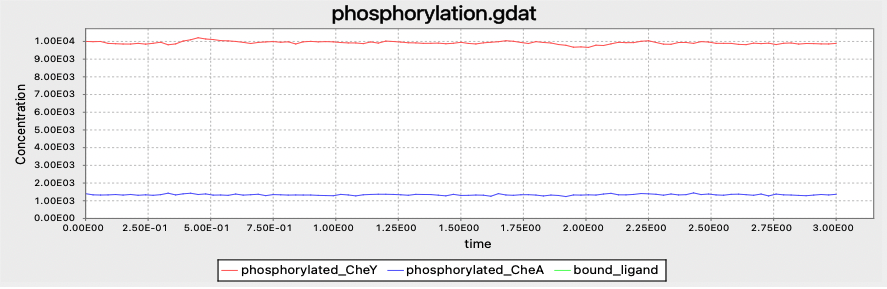
\includegraphics[width = 0.85\textwidth]{../images/chemotaxis_tutorial5.png}
\caption{Molecular concentrations (in number of molecules in the cell) over time (in seconds) in a BioNetGen chemotaxis simulation in which no ligand is present.}
\label{fig:chemotaxis_tutorial5}
\end{figure}

The sudden addition of 5,000 attractant ligand molecules increases the concentration of bound receptors, therefore leading to less CheA autophosphorylation, and less phosphorylated CheY (\autoref{fig:chemotaxis_tutorial6}).\\

\begin{figure}[h]
\centering
\mySfFamily
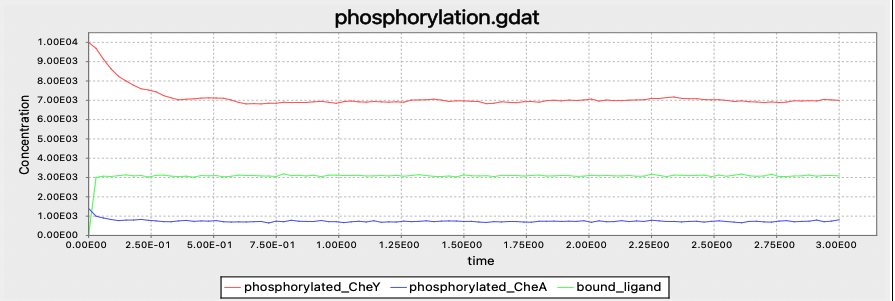
\includegraphics[width = 0.85\textwidth]{../images/chemotaxis_tutorial6.png}
\caption{Molecular concentrations (in number of molecules in the cell) over time (in seconds) in a BioNetGen chemotaxis simulation with 5,000 initial attractant ligand particles.}
\label{fig:chemotaxis_tutorial6}
\end{figure}

If we instead add 100,000 attractant molecules, then we see an even more drastic decrease in phosphorylated CheA and CheY (\autoref{fig:chemotaxis_tutorial7}).

\begin{figure}[h]
\centering
\mySfFamily
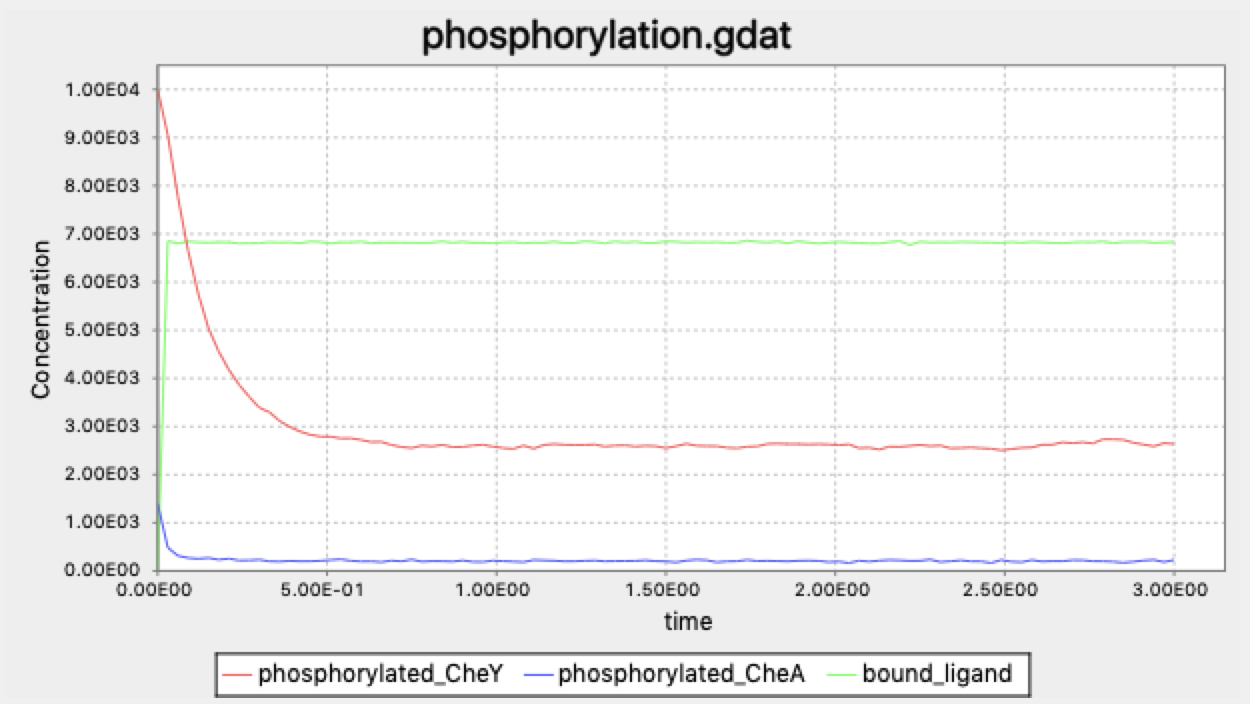
\includegraphics[width = 0.85\textwidth]{../images/chemotaxis_tutorial7.png}
\caption{Molecular concentrations (in number of molecules in the cell) over time (in seconds) in a BioNetGen chemotaxis simulation with 100,000 initial attractant ligand particles.}
\label{fig:chemotaxis_tutorial7}
\end{figure}


In other words, the BioNetGen simulation is confirming that an increase in attractant reduces the concentration of phosphorylated CheY, which therefore lowers the tumbling frequency. What is remarkable about this is how quickly it takes place, with the cell attaining a new equilibrium in a fraction of a second.


\FloatBarrier
\phantomsection
\subsection{So \ldots what's the big deal?}

You may not be surprised that we have been able to build a simple model of the response of \textit{E. coli} to an attractant ligand. After all, the biochemistry presented here may be elegant, but it is also simple.

But what we have shown in this section is just part of the story. In the next section, we will see that the biochemical realities of chemotaxis are even more complicated, and for good reason --- this added complexity will allow \textit{E. coli} to react to a dynamic world with surprising sophistication.\\

\FloatBarrier
\phantomsection

\section{Methylation Helps a Bacterium Adapt to Differing Concentrations}
\label{sec:methylation}

\phantomsection
\subsection{Bacterial tumbling frequencies remain constant for different attractant concentrations}

Earlier in this chapter, we explored the signal transduction pathway by which \textit{E. coli} can change its tumbling frequency in response to a change in the concentration of an attractant. But the reality of cellular environments is that the concentration of an attractant can vary across several orders of magnitude. The cell therefore needs to detect not \textit{absolute} concentrations of an attractant but rather \textit{relative} changes.

\textit{E. coli} detects relative changes in its concentration via \textdefnogloss{adaptation} to the signal concentration. If the concentration of attractant remains constant for a period of time, then regardless of the absolute value of the concentration, the cell returns to the same background tumbling frequency. In other words, \textit{E. coli} demonstrates \textit{robustness} to the background concentration of attractant in maintaining its default tumbling behavior.

However, our current model is not able to address this adaptation. If the ligand concentration increases, then phosphorylated CheY plummets. But if the ligand concentration remains elevated, then the bacterium should eventually resume its exploration. In our model, CheY would remain at a low steady state, and tumbling frequency would be low.

In this section, we will investigate the biochemical mechanism that \textit{E. coli} uses to achieve such a robust response to environments with different background concentrations. We will then further expand the model we built in the previous section to see if this model can replicate the bacterium's adaptive response.

\FloatBarrier
\phantomsection
\subsection{Bacteria remember past concentrations using methylation}

Recall that in the absence of an attractant, CheW and CheA readily bind to an MCP, leading to greater autophosphorylation of CheA, which in turn phosphorylates CheY. The greater the concentration of phosphorylated CheY, the more frequently the bacterium tumbles.

Signal transduction is achieved through phosphorylation, but \textit{E. coli} maintains a ``memory'' of past environmental concentrations through a chemical process called \textdef{methylation}{methylation}{a chemical reaction in which a methyl group ($-\text{CH}_3$) is added to an organic molecule}. In this reaction, a \textdefnogloss{methyl group} ($-\text{CH}_3$) is added to an organic molecule; the removal of a methyl group is called \textdef{demethylation}{demethylation}{the reversal of a methylation reaction, in which a methyl group ($-\text{CH}_3$) is removed from an organic molecule}.

Every MCP receptor contains four methylation sites, meaning that between zero and four methyl groups can be added to the receptor. On the plasma membrane, many MCPs, CheW, and CheA molecules form an array structure. Methylation reduces the negative charge on the receptors, stabilizing the array and facilitating CheA autophosphorylation. The more sites that are methylated, the higher the autophosphorylation rate of CheA, which means that CheY has a higher phosphorylation rate, and tumbling frequency increases.

We now have two different ways that tumbling frequency can be elevated. First, if the concentration of an attractant is low, then CheW and CheA freely form a complex with the MCP, and the phosphorylation cascade passes phosphoryl groups to CheY, which interacts with the flagella and keeps tumbling frequency high. Second, an increase in MCP methylation can also boost CheA autophosphorylation and lead to an increased tumbling frequency.

Methylation of MCPs is achieved by an additional protein called \textbf{CheR}. When bound to MCPs, CheR methylates ligand-bound MCPs faster, and so the rate of MCP methylation by CheR is higher if the MCP is bound to a ligand. Let's consider how this fact affects a bacterium's behavior.

Say that \textit{E. coli} encounters an increase in attractant concentration. Then the lack of a phosphorylation cascade will mean less phosphorylated CheY, and so the tumbling frequency will decrease. However, if the attractant concentration levels off, then the tumbling frequency will flatten, while CheR starts methylating the MCP. Over time, the rising methylation will increase CheA autophosphorylation, bringing back the phosphorylation cascade and raising tumbling frequency back to default levels.

Just as the phosphorylation of CheY can be reversed, MCP methylation can be undone to prevent methylation from being permanent. In particular, an enzyme called \textbf{CheB}, which like CheY is phosphorylated by CheA, demethylates MCPs (as well as autodephosphorylates). The rate of an MCP's demethylation is dependent on the extent to which the MCP is methylated. In other words, the rate of MCP methylation is higher when the MCP is in a low methylation state, and the rate of demethylation is faster when the MCP is in a high methylation state.

\autoref{fig:chemotaxis_wholestory} adds CheR and CheB to provide a complete picture of the core pathways influencing chemotaxis. To model these pathways, we will need to add quite a few molecules and reactions to our current model.\\

\begin{figure}[h]
\centering
\mySfFamily
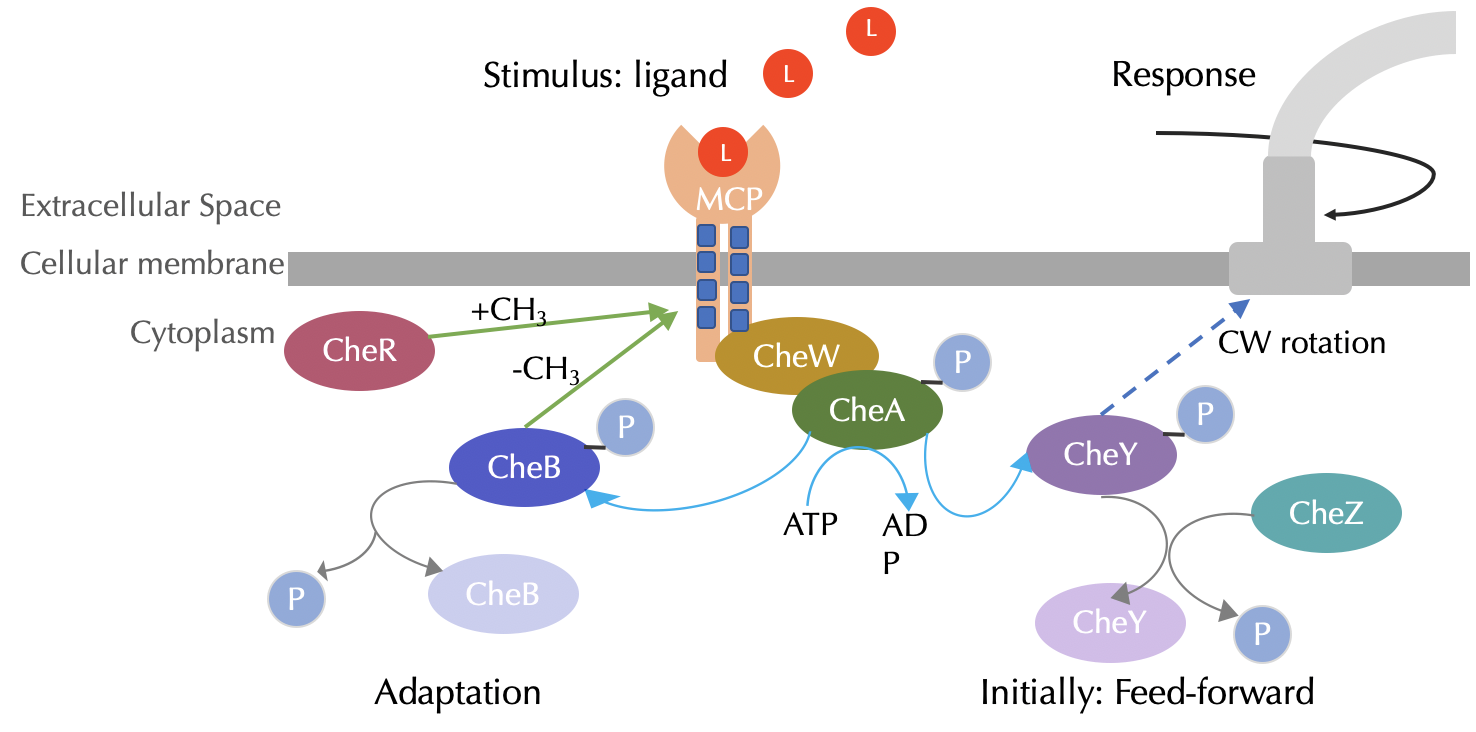
\includegraphics[width = 0.85\textwidth]{../images/chemotaxis_wholestory.png}
\caption{The chemotaxis signal-transduction pathway with methylation included. CheA phosphorylates CheB, which methylates MCPs while CheR demethylates MCPs. Blue lines denote phosphorylation, grey lines denote dephosphorylation, green arrows denote methylation, and red arrows denote demethlyation. Image modified from \href{http://chemotaxis.biology.utah.edu/Parkinson_Lab/projects/ecolichemotaxis/ecolichemotaxis.html}'s illustrations.}
\label{fig:chemotaxis_wholestory}
\end{figure}


\FloatBarrier
\phantomsection
\subsection{Combinatorial explosion and the need for rule-based modeling}

We would like to add the methylation reactions discussed above to the model that we built in the previous section and see if this model can replicate the adaptation behavior of \textit{E. coli} in the presence of a changing attractant concentration. Before incorporating the adaptation mechanisms in our BioNetGen model, we will first describe the reactions that BioNetGen will need.

We begin with considering the MCP complexes. In a tutorial, \tutorial[https://biologicalmodeling.org/chemotaxis/tutorial_phos] we identified two components relevant for reactions involving MCPs: a ligand-binding component \texttt{;} and a phosphorylation component \texttt{Phos}. The adaptation mechanism introduces two additional reactions: methylation of the MCP by CheR, and demethylation of the MCP by CheB.

We also need to include binding and dissociation reactions between the MCP and CheR because under normal conditions, most CheR are bound to MCP complexes. We will therefore introduce two additional components to the MCP molecules in addition to their phosphorylation components: \texttt{r} (denoting CheR-binding) and \texttt{Meth} (denoting methylation states). In our simulation, we will use three methylation levels (low, medium, and high) rather than five because these three states are most involved in the chemotaxis response to attractants.

Imagine for a moment that we were attempting to specify every reaction that could take place in our model. To specify an MCP, we would need to tell the program whether it is bound to a ligand (two possible states), whether it is bound to CheR (two possible states), whether it is phosphorylated (two possible states), and which methylation state it is in (three possible states). Therefore, a given MCP has $2 \cdot 2 \cdot 2 \cdot 3 = 24$ total states.

Say that we are simulating the simple reaction of a ligand binding to an MCP, which we originally wrote as $T + L \rightarrow TL$. We now need this reaction to include 12 of the 24 states, the ones corresponding to the MCP being unbound to the ligand. Our previously simple reaction would become 12 different reactions, one for each possible unbound state of the complex molecule $T$. And if the situation were just a little more complex, with the ligand molecule $L$ having $n$ possible states, then we would have $12n$ reactions. Imagine trying to debug a model in which we had accidentally incorporated a typo when transcribing just one of these reactions!

In other words, as our model grows, with multiple different states for each molecule involved in each reaction, the number of reactions we need to represent the system grows very fast; this phenomenon is called \textdef{combinatorial explosion}{combinatorial explosion}{a phenomenon in which the complexity of a problem grows rapidly due to the growth in the number of some quantity of interest (e.g., the number of possible reactions in a molecular system)}. Our model of chemotaxis is ultimately relatively straightforward, but combinatorial explosion means that building realistic models of biochemical systems at scale can be daunting.

A major benefit of using a rule-based modeling language such as the one developed by BioNetGen is that it circumvents combinatorial explosion by consolidating many reactions into a single rule. For example, when modeling ligand-MCP binding, we can summarize the 12 different reactions with the rule ``a free ligand molecule binds to an MCP that is not bound to a ligand molecule.'' In the BioNetGen language, this rule is represented by the same one-line expression as it was in the previous section:

\begin{verbatim}
LigandReceptor: L(t) + T(l) <-> L(t!1).T(l!1) k\_lr\_bind, k\_lr\_dis
\end{verbatim}

We will not bog down the text with a full specification of all the rules needed to add methylation to our model while avoiding combinatorial explosion. If you're interested in the details, please follow our tutorial \tutorial[https://biologicalmodeling.org/chemotaxis/tutorial_adaptation].


\FloatBarrier
\phantomsection
\subsection{Bacterial tumbling is robust to large sudden changes in attractant concentration}

In the figures that follow, we show plots of the concentration of each molecule of interest in our system for a few different cases. In each case, we suddenly change the concentration of the attractant ligand $l_0$ and examine how this affects the concentration of phosphorylated CheY. The attractant concentration will then level off; how will our model respond?

Below, we show simulation results for some different concentrations of ligand molecules added at the beginning of the simulation. First we add a relatively small amount of attractant, setting $l_0$ equal to 10,000. The system returns so quickly to an equilibrium in phosphorylated CheY that it is difficult to imagine that the attractant has had any effect on tumbling frequency.

\begin{figure}[h]
\centering
\mySfFamily
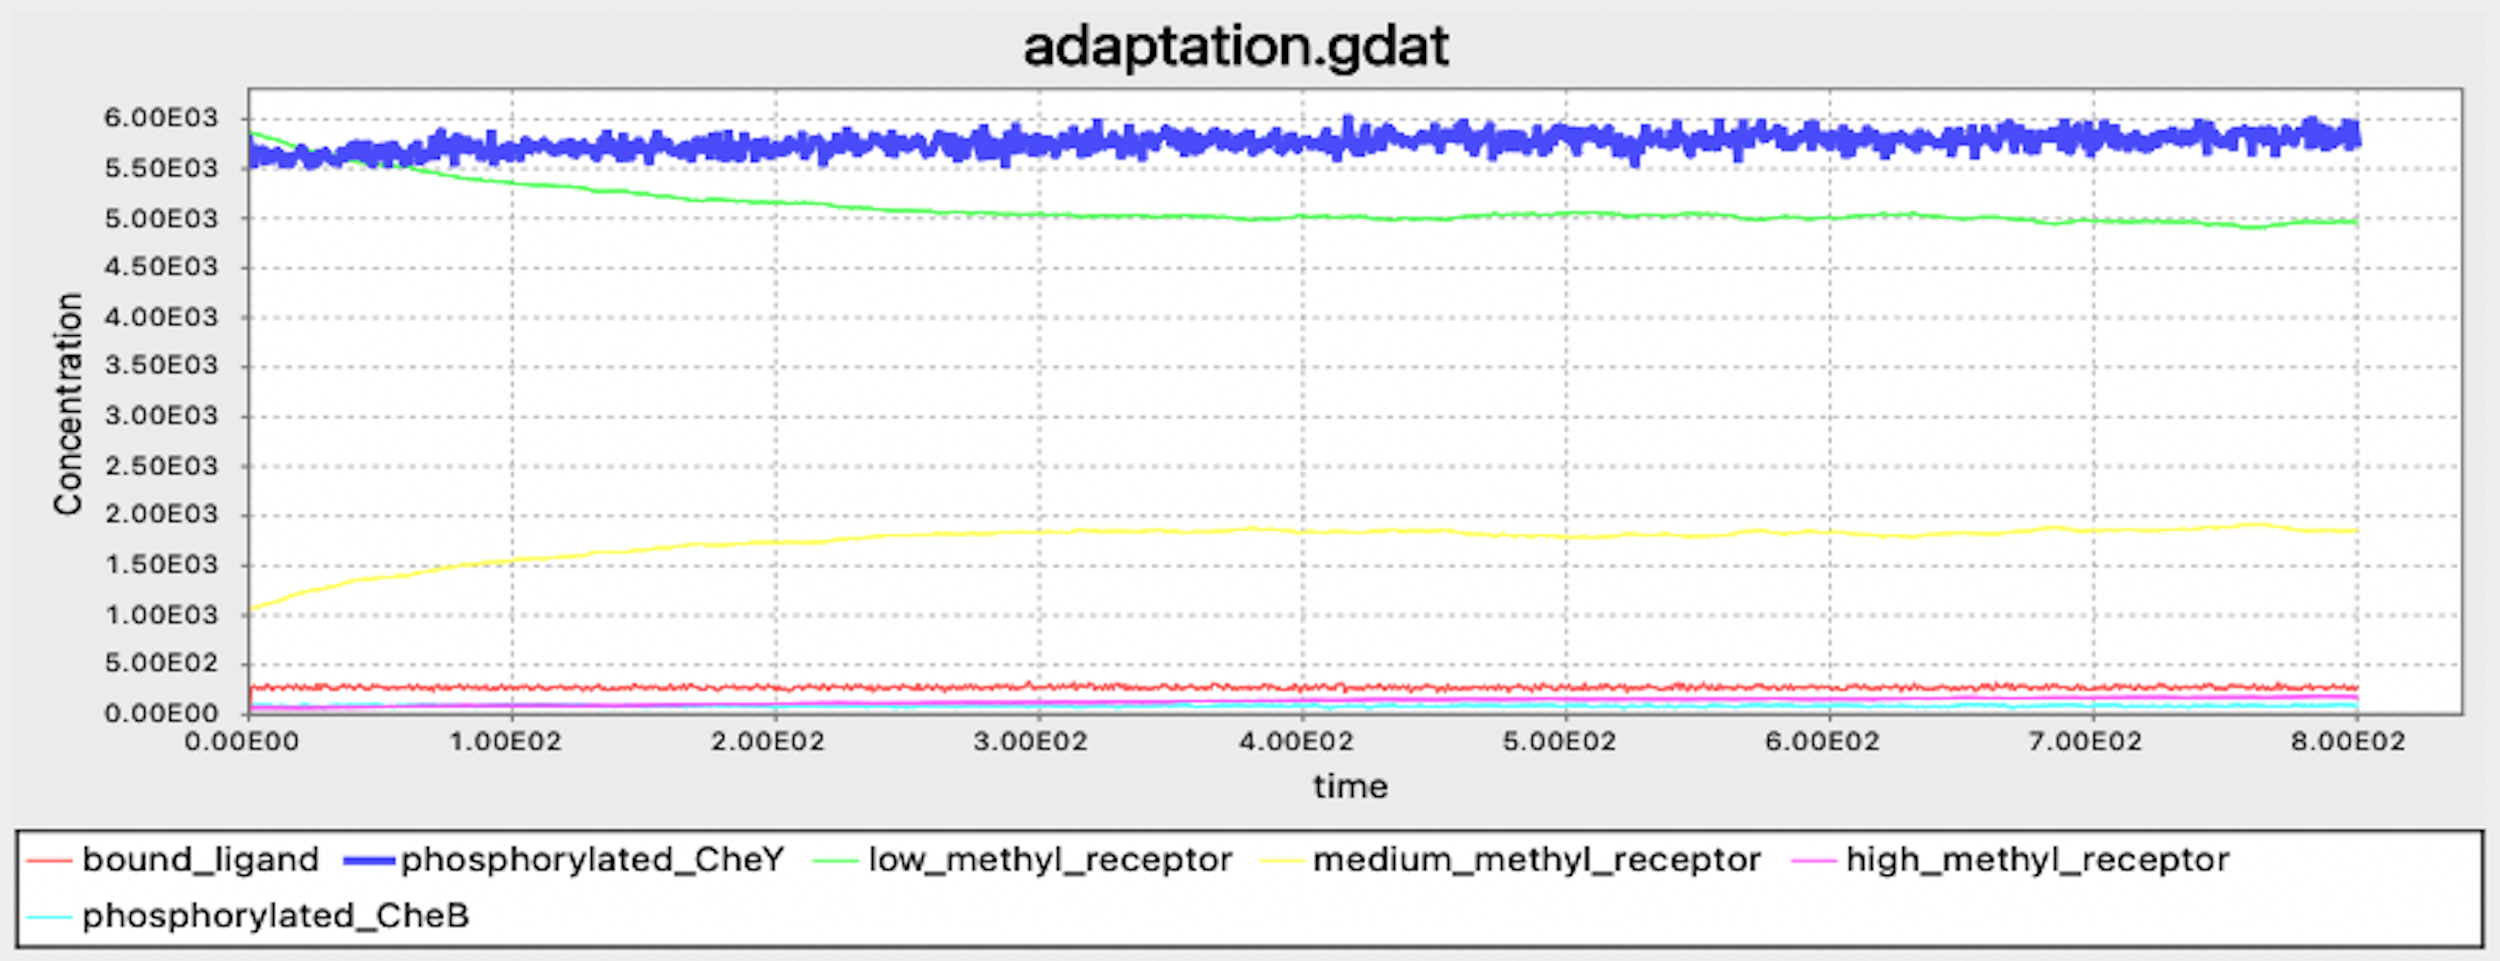
\includegraphics[width = 0.85\textwidth]{../images/chemotaxis_tutorial_oneadd1e4.png}
\caption{Molecular concentrations (in number of molecules in the cell) over time (in seconds) in a BioNetGen chemotaxis simulation with 10,000 initial attractant ligand particles.}
\label{fig:chemotaxis_tutorial_oneadd1e4}
\end{figure}


If instead $l_0$ is equal to 100,000, then we obtain the result in \autoref{fig:chemotaxis_tutorial_oneadd1e5}. After an initial drop in the concentration of phosphorylated CheY, it returns to equilibrium after a few minutes.

\begin{figure}[h]
\centering
\mySfFamily
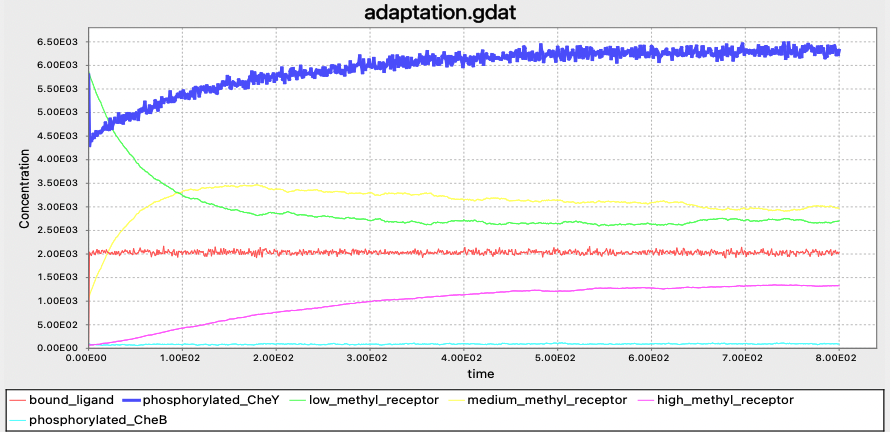
\includegraphics[width = 0.85\textwidth]{../images/chemotaxis_tutorial_oneadd1e5.png}
\caption{Molecular concentrations (in number of molecules in the cell) over time (in seconds) in a BioNetGen chemotaxis simulation with 100,000 initial attractant ligand particles.}
\label{fig:chemotaxis_tutorial_oneadd1e5}
\end{figure}


When we increase $l_0$ by another factor of ten to 1 million, the initial drop is more pronounced, but the system returns just as quickly to equilibrium. Note how much higher the concentration of methylated receptors are in \autoref{fig:chemotaxis_tutorial_oneadd16} compared to \autoref{fig:chemotaxis_tutorial_oneadd1e5}; however, there are still a significant concentration of receptors with low methylation, indicating that the system may be able to handle an even larger jolt of attractant.\\

\begin{figure}[h]
\centering
\mySfFamily
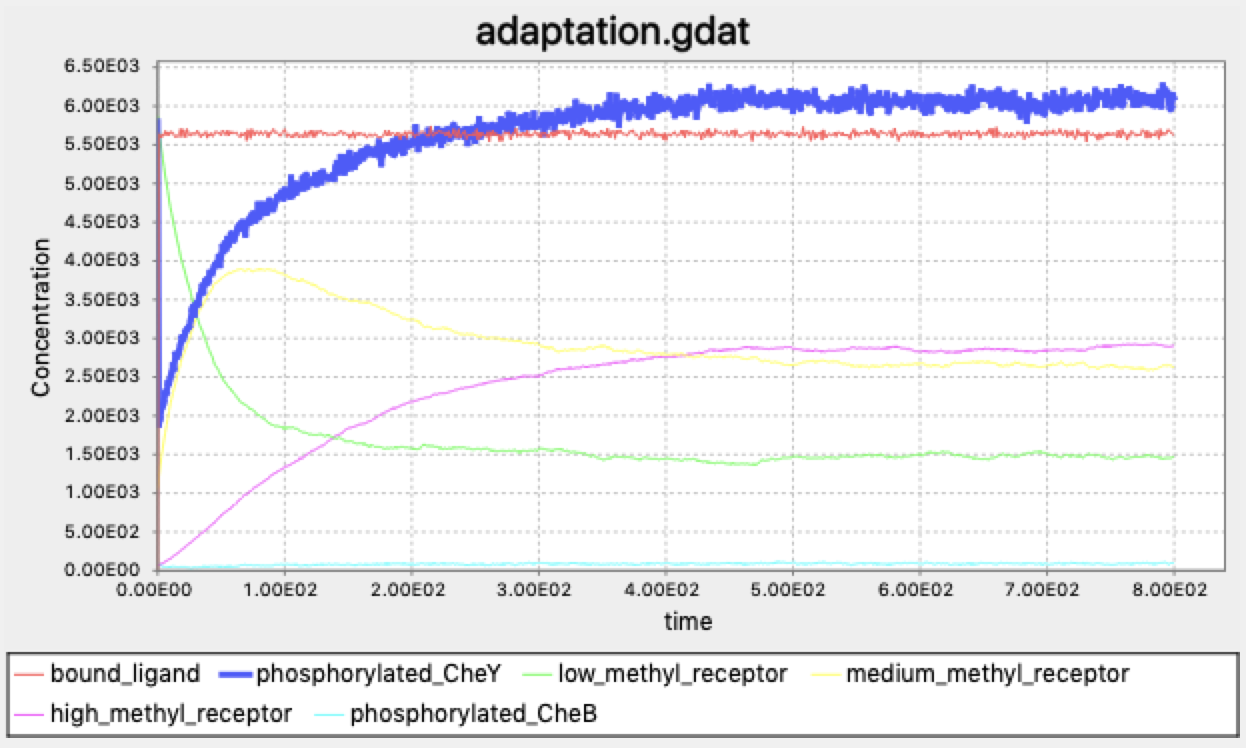
\includegraphics[width = 0.85\textwidth]{../images/chemotaxis_tutorial_oneadd1e6.png}
\caption{Molecular concentrations (in number of molecules in the cell) over time (in seconds) in a BioNetGen chemotaxis simulation with one million initial attractant ligand particles.}
\label{fig:chemotaxis_tutorial_oneadd16}
\end{figure}

When we set $l_0$ equal to 10 million, we give the system this bigger jolt. Once again, the model returns to its previous CheY equilibrium after a few minutes (\autoref{fig:chemotaxis_tutorial_oneadd1e7}).

\begin{figure}[h]
\centering
\mySfFamily
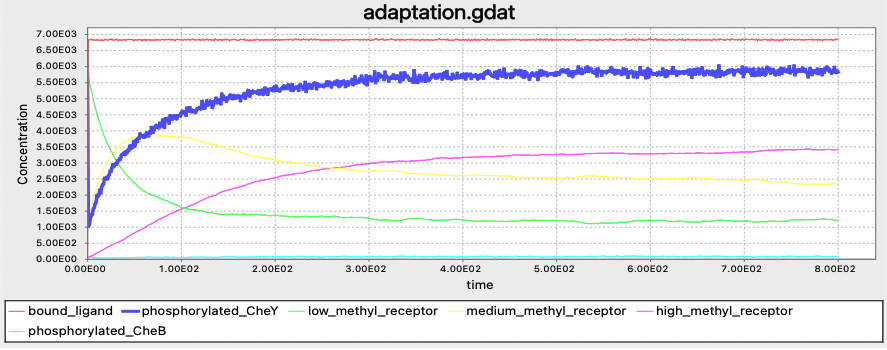
\includegraphics[width = 0.85\textwidth]{../images/chemotaxis_tutorial_oneadd1e7.png}
\caption{Molecular concentrations (in number of molecules in the cell) over time (in seconds) in a BioNetGen chemotaxis simulation with ten million initial attractant ligand particles.}
\label{fig:chemotaxis_tutorial_oneadd1e7}
\end{figure}

Finally, with $l_0$ equal to 100 million, we see what we might expect: the steepest drop in phosphorylated CheY yet, but a system that is able to return to equilibrium (\autoref{fig:chemotaxis_tutorial_oneadd1e8}).

\begin{figure}[h]
\centering
\mySfFamily
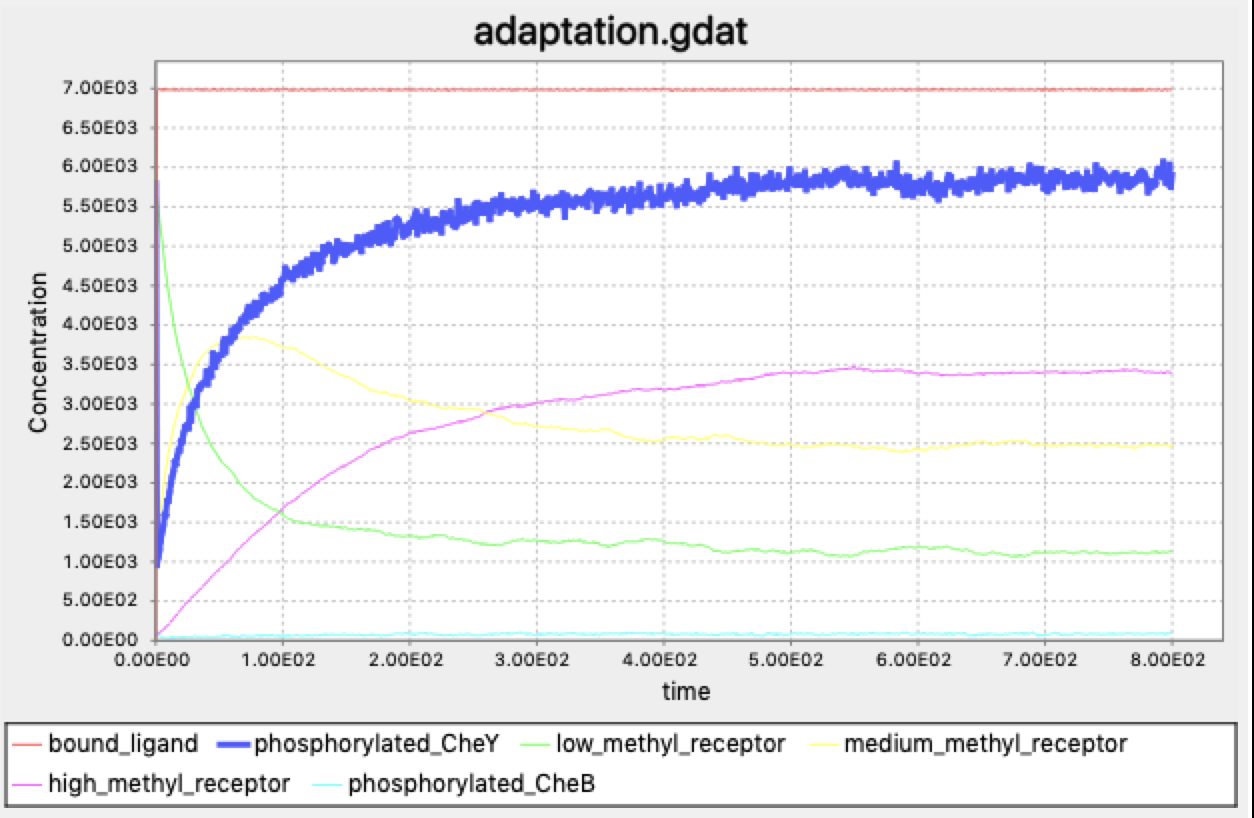
\includegraphics[width = 0.85\textwidth]{../images/chemotaxis_tutorial_oneadd1e8.png}
\caption{Molecular concentrations (in number of molecules in the cell) over time (in seconds) in a BioNetGen chemotaxis simulation with 100 million initial attractant ligand particles.}
\label{fig:chemotaxis_tutorial_oneadd1e8}
\end{figure}

Our model, which is built on real reaction rate parameters, provides compelling evidence that the \textit{E. coli} chemotaxis system is very robust to changes in its environment. Our simulated bacterium can make a very rapid change in response to a sudden change in its environment, but even if this change is significant, the system will return to its default state. This robustness in our simulation has been observed in real bacteria , as well as replicated by other computational simulations.

Aren't bacteria magnificent?

However, our work is not done. We have simulated \textit{E. coli} adapting to a single sudden change in its environment, but life is about responding to continual change. So in the next section, we will further examine how our simulated bacterium responds in an environment in which the ligand concentration is changing constantly.\\


\FloatBarrier
\phantomsection

\section{Modeling a Bacterium's Response to an Attractant Gradient}
\label{sec:gradient}

\phantomsection
\subsection{Traveling up an attractant gradient}

Earlier, we saw that \textit{E. coli} is able to adapt its default tumbling frequency to the current background concentration of attractant. To model this behavior, we used the Gillespie algorithm and the rule-based language of BioNetGen to simulate an instantaneous increase in concentration from one stable concentration level to another.

Yet imagine a glucose cube in an aqueous solution. As the cube dissolves, a \textdefnogloss{gradient} will form, with a glucose concentration that decreases outward from the cube. How will the tumbling frequency of \textit{E. coli} change if the bacterium finds itself in an environment of an attractant gradient?  Will the tumbling frequency decrease continuously as well, or will the methylation pathways mentioned in the previous section cause more complicated behavior? And once the cell reaches a region of high attractant concentration, will its default tumbling frequency stabilize to the same steady state?

In this section, we will modify our model from the previous section by increasing the concentration of the attractant ligand at an exponential rate and seeing how the concentration of phosphorylated CheY changes. This model will simulate a bacterium traveling up an attractant gradient toward an attractant. Moreover, we will examine how the concentration of phosphorylated CheY changes as we change the gradient's ``steepness'', or the rate at which attractant ligand is increasing. Visit the following tutorial \tutorial[https://biologicalmodeling.org/chemotaxis/tutorial_gradient] if you're interested in following our adjustments for yourself.

\phantomsection
\subsection{Steady state tumbling frequency is robust}

Recall that we used the expression $[L]$ to denote the concentration of ligand $L$ and $l_0$ to denote the initial concentration of the ligand. To model a ligand concentration that is increasing exponentially, we will use the function $[L] = l_0 \cdot e^{k \cdot t}$, where $t$ is the time and $k$ is a parameter dictating exponential growth. The parameter $k$ represents the steepness of the gradient, since the higher the value of $k$, the faster the growth in the ligand concentration.

For example, \autoref{fig:chemotaxis_tutorial_addition01} shows the concentration over time of phosphorylated CheY (shown in blue) when $l_0 = 1000$ and $k = 0.1$. The concentration of phosphorylated CheY, and therefore the tumbling frequency, still decreases sharply as the ligand concentration increases, but after all ligands become bound to receptors (shown by the plateau in the red curve), the methylation of receptors causes the concentration of phosphorylated CheY to return to its equilibrium. In other words, for these values of $l_0$ and $k$, the outcome is similar to when we provided an instantaneous increase in ligand, although the cell takes longer to reach its minimum concentration of phosphorylated CheY because the attractant concentration is increasing gradually.\\

\begin{figure}[h]
\centering
\mySfFamily
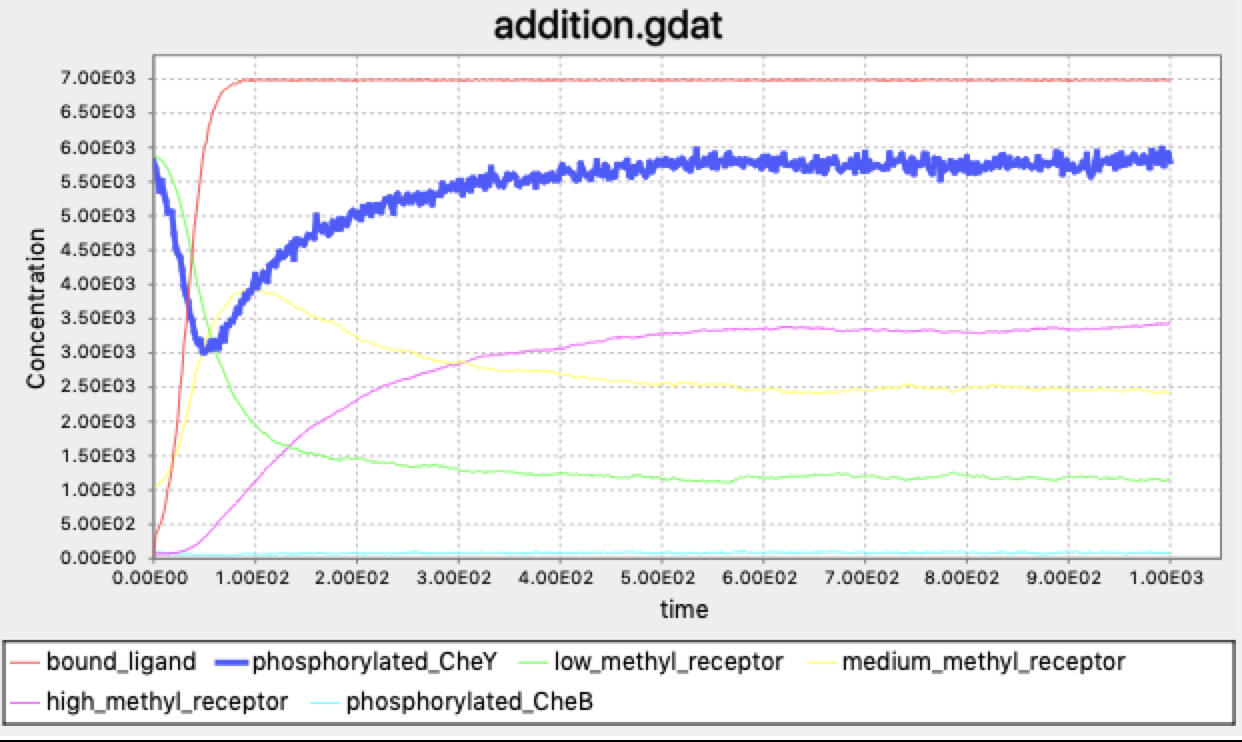
\includegraphics[width = 0.85\textwidth]{../images/chemotaxis_tutorial_addition01.png}
\caption{Plots of relevant molecule concentrations in our model (in number of molecules in the cell) over time (in seconds) when the concentration of ligand grows exponentially with $\textvar{l}_\text{0} = \text{1000}$ and $\textvar{k} = \text{0.1}$. The concentration of bound ligand (shown in red) quickly hits saturation, which causes a minimum in phosphorylated CheY (and therefore a low tumbling frequency). To respond, the cell increases the methylation of receptors, which boosts the concentration of phosphorylated CheY back to equilibrium.}
\label{fig:chemotaxis_tutorial_addition01}
\end{figure}


Our next question is what happens as we change $k$, the growth rate of the ligand concentration. \autoref{fig:chemotaxis_tutorial_addition03} shows the results of multiple simulations in which we vary the growth parameter $k$ and plot the concentration of phosphorylated CheY over time. The larger the value of $k$, the faster the increase in receptor binding, and the steeper the drop in the concentration of phosphorylated CheY.\\

\begin{figure}[h]
\centering
\mySfFamily
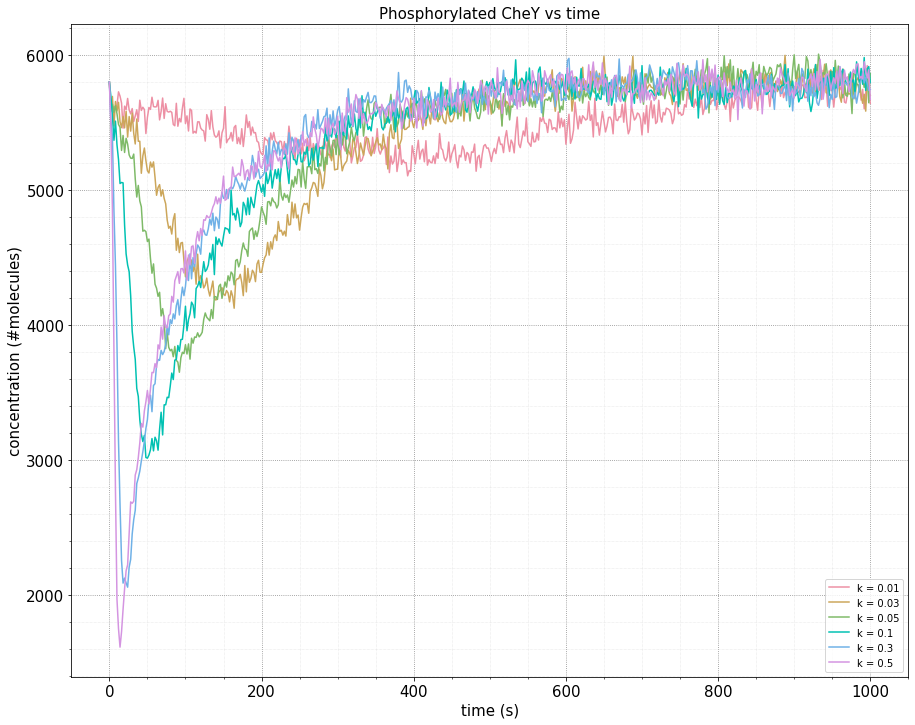
\includegraphics[width = 0.85\textwidth]{../images/chemotaxis_tutorial_addition03.png}
\caption{Plots of phosphorylated CheY for different growth rates \textvar{k} of the concentration of ligand. The larger the value of \textvar{k}, the steeper the initial drop as the concentration of bound ligand becomes saturated, and the faster the concentration of phosphorylated CheY returns to equilibrium.}
\label{fig:chemotaxis_tutorial_addition03}
\end{figure}

More importantly, \autoref{fig:chemotaxis_tutorial_addition03} further illustrates the \textit{robustness} of bacterial chemotaxis to the rate of growth in ligand concentration. Whether the growth of the attractant is slow or fast, methylation will always bring the cell back to the same equilibrium concentration of phosphorylated CheY, and therefore the same background tumbling frequency.

\FloatBarrier
\phantomsection
\subsection{Reversing the attractant gradient}

And what if a cell is moving away from an attractant, down a concentration gradient? We would hope that the cell would be able to \textit{increase} its tumbling frequency (i.e., increase the concentration of phosphorylated CheY), and then restore the background tumbling frequency by removing methylation.

To simulate a decreasing gradient, we will model a cell in a high ligand concentration that is already at steady state, meaning that methylation is also elevated. In this case, the ligand concentration will \textit{decay} exponentially, meaning that the ligand concentration is still given by the equation $\text{[}L{]} = l_0 \cdot e^{k \cdot t}$, but $k$ is negative.\\

\begin{qbox}[%
If $k$ is negative, how do you think that decreasing the value of $k$ will affect the concentration of phosphorylated CheY over time?
]\end{qbox}

You may like to modify the previous tutorial on your own to account for traveling down an attractant gradient. If not, we are still happy to provide a separate tutorial \tutorial[https://biologicalmodeling.org/chemotaxis/tutorial_removal].


\FloatBarrier
\phantomsection
\subsection{Steady state tumbling frequency remains robust when traveling down an attractant gradient}

\autoref{fig:chemotaxis_tutorial_removal01} plots the concentrations of molecules in our model as the concentration of attractant ligand decreases exponentially with $l_0$ equal to $10^7$ and $k$ equal to $-0.3$. As the ligand concentration decreases, the concentration of bound ligands plummet as bound ligands dissociate and there are not enough free ligands to replace the dissociating ones. In the absence of ligand-receptor binding, CheY is free to phosphorylate, causing a spike in phosphorylated CheY. Demethylation of receptors then causes the concentration of phosphorylated CheY to steadily return back to its equilibrium.\\

\begin{figure}[h]
\centering
\mySfFamily
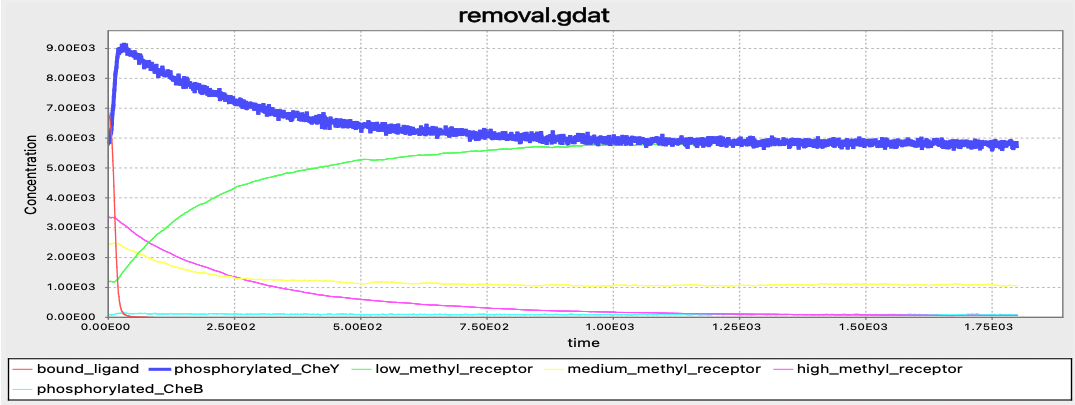
\includegraphics[width = 0.85\textwidth]{../images/chemotaxis_tutorial_removal01.png}
\caption{Molecular concentrations (in number of molecules in the cell) over time (in seconds) for a simulated bacterium traveling down an attractant gradient with $\textvar{l}_\text{0} = \text{10}^\text{7}$ and \textvar{k} equal to $-\text{0.3}$. Phosphorylated CheY follows the opposite pattern to traveling up an attractant gradient, with the concentration of phosphorylated CheY rising quickly only to slowly decrease to equilibrium due to demethylation.}
\label{fig:chemotaxis_tutorial_removal01}
\end{figure}


To be thorough, we should also test the robustness of our model to see whether the CheY concentration will return to the same steady state for a variety of values of $k$ when $k$ is negative. As in the case of an increasing gradient, \autoref{fig:chemotaxis_tutorial_removal02} shows that the more sudden the change in the concentration of attractant (i.e., the more negative the value of $k$), the sharper the spike. And yet regardless of the value of $k$, methylation does its work to bring the concentration back to the same steady state, which has been confirmed by experimental observations.\\

\begin{figure}[h]
\centering
\mySfFamily
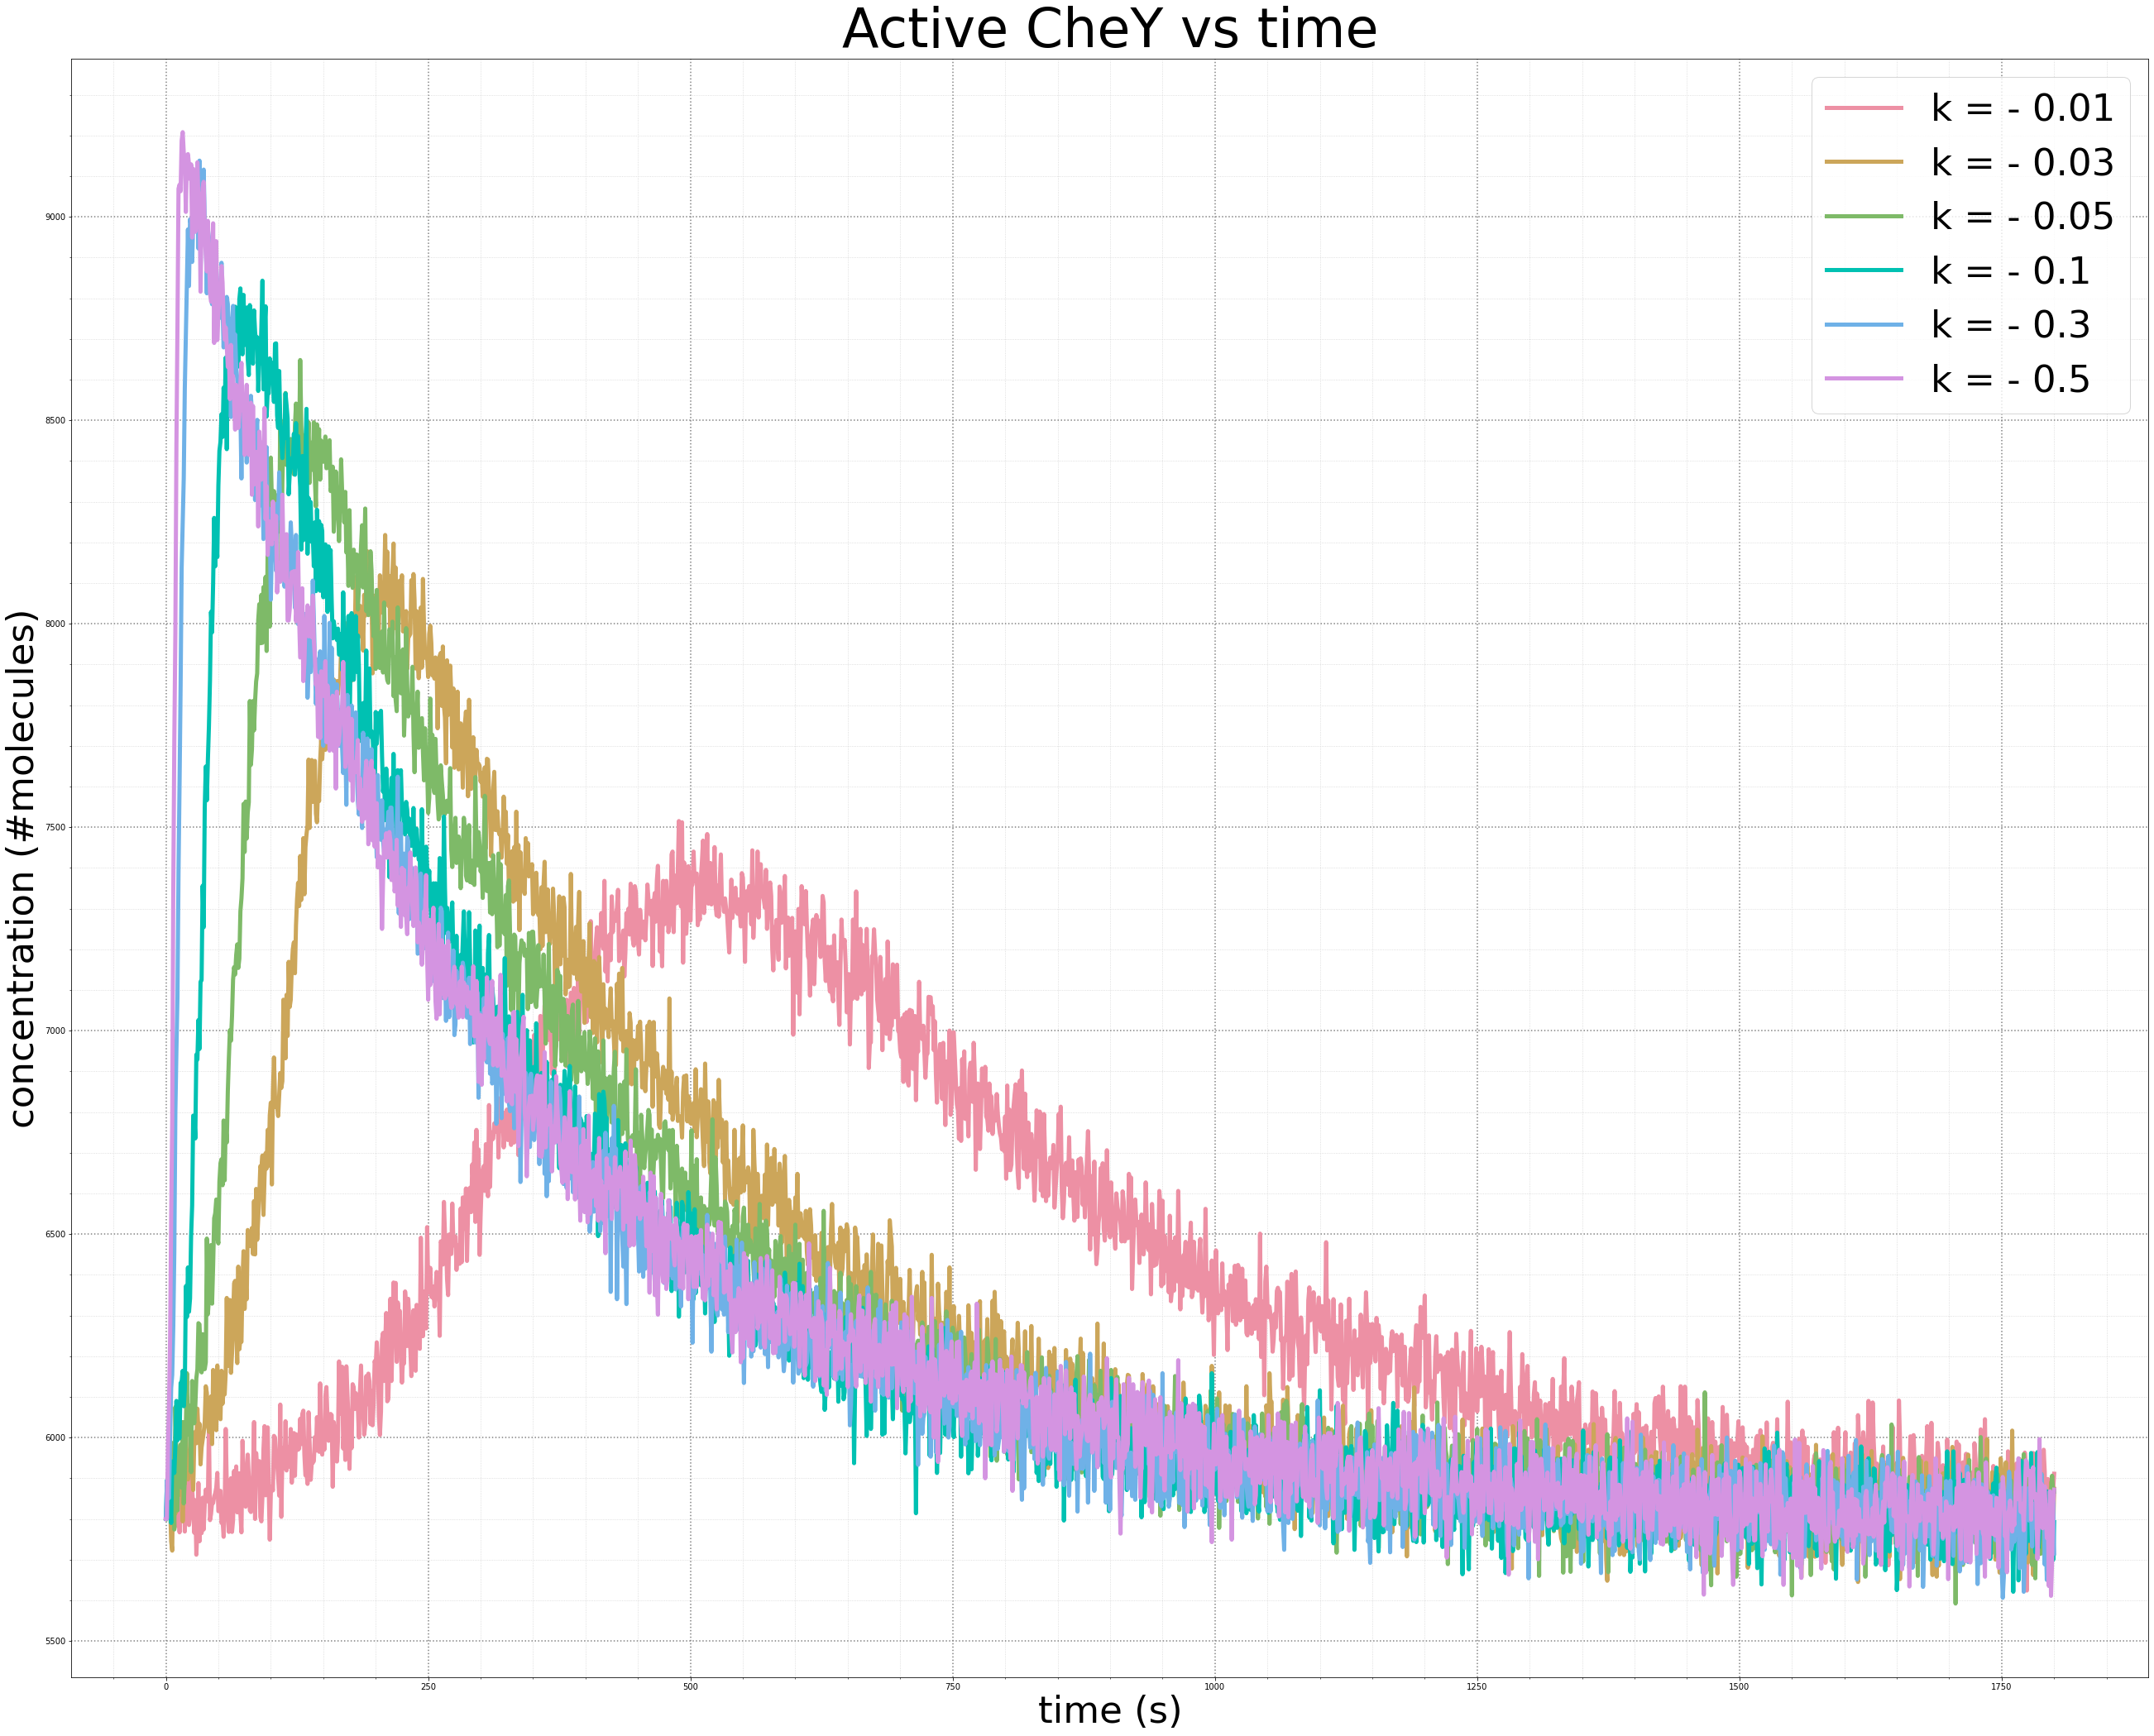
\includegraphics[width = 0.85\textwidth]{../images/chemotaxis_tutorial_removal02.png}
\caption{Varying values of \textvar{k} in our exponential decrease in the concentration of attractant ligand produce the same equilibrium concentration of phosphorylated CheY. The smaller the value of \textvar{k}, the steeper the initial spike, and the faster the recovery to steady state.}
\label{fig:chemotaxis_tutorial_removal02}
\end{figure}

\phantomsection
\subsection{From changing tumbling frequencies to an exploration algorithm}

We hope that you have gained an appreciation for the elegant mechanism of bacterial chemotaxis, as well as the power of rule-based modeling and the Gillespie algorithm for simulating a complex biochemical system with a huge number of reactions without the need to keep track of individual particles.

And yet we have missed an important part of the story. \textit{E. coli} has evolved to ensure that if it detects a relative increase in concentration (i.e., an attractant gradient), then it can reduce its tumbling frequency in response. But what we have not explored is \textit{why} this change in the bacterium's tumbling frequency would help it find food in the first place.

After all, according to the run and tumble model, the direction that a bacterium is moving at any point in time is random! So why would a decrease in tumbling frequency help \textit{E. coli} move toward an attractant?

This question is biologically deep and has no immediate intuitive answer. However, in this chapter's conclusion, we will build a model to explain why \textit{E. coli}'s run and tumble walk algorithm is an extremely clever way of locating resources in an unfamiliar land.\\


\FloatBarrier
\phantomsection

\section{Conclusion: The Beauty of \textit{E. coli}'s Robust Randomized Exploration Algorithm}
\label{sec:conclusion}

\phantomsection
\subsection{Two randomized exploration strategies}

In \autoref{chapter:turing}, we saw that a particle taking a collection of \textit{n} unit steps in random directions will wind up on average $\sqrt{n}$ distance away from its starting position. We now would like to compare this random walk against a modified version of the walk that emulates the behavior of \textit{E. coli} that we have learned about in this chapter.

Specifically, we will place a particle against a background containing a variable concentration of attractant. The bacterium will reorient itself randomly, but it will be able to change its tumbling frequency based on the relative concentration of attractant at its current location. Does this realistic exploration algorithm allow the bacterium to find attractant faster than a pure random walk strategy?

We will represent a bacterium as a point in two-dimensional space. Units in our space will be measured in µm, so that moving from (0, 0) to (0, 20) is 20µm, a distance that we know from the introduction can be covered by the bacterium in 1 second during an uninterrupted run. The bacterium will start at the \textbf{origin} (0, 0), which we will establish to have a ligand concentration of 100 molecules/µm\textsuperscript{3}.

We will use $L(x,y)$) to denote the ligand concentration at ($x$, $y$); furthermore, we simulate an attractant gradient by ensuring that there is a point (called the \textbf{goal}) at which $L(x,y)$) is maximized. We will set the concentration at the goal equal to 10\textsuperscript{8} molecules/µm\textsuperscript{3}, and we will place the goal at $(\text{1,500}, \text{1,500})$, so that the bacterium must travel a significant distance to find the attractant.

We would like the ligand concentration $L(x,y)$) to decrease exponentially the farther we travel from the goal. We therefore set $L(x,y)$) = $100 \cdot 10^{6 \cdot (1-d/D)}$, where $d$ is the distance from ($x$, $y$) to the goal, and $D$ is the distance from the origin to the goal, which in this case is $\
text{1,500}\sqrt{2} \approx 2121$ µm.\\

\begin{qbox}[%
How can we quantify how well a bacterium has done at finding the attractant?
]\end{qbox}

For each of our two strategies, we will simulate many random walks of a given bacterium throughout this space for a fixed time. (The total time needed by our simulation should be large enough to allow the bacterium to have enough time to reach the goal.) To compare the two strategies, we will then measure how far \textit{on average} a bacterium with each strategy is from the goal at the end of the simulation.

We will now implement each of the two exploration strategies that we wish to model.\\

\FloatBarrier
\phantomsection
\subsection{Strategy 1: Standard random walk}

To model our ``unintelligent'' random walk strategy, we first select a random direction of movement along with a duration of tumble. The degree of reorientation follows a uniform distribution from 0° to 360°. The duration of each tumble follows an exponential distribution with mean 0.1\textvar{s}. As the result of a tumble, the cell only changes its orientation, not its position.

We then select a random duration to run and let the bacterium run in that direction for the specified amount of time. The duration of each run follows an exponential distribution with mean equal to the experimentally verified value of 1 second.

We then iterate these two steps of tumbling and running until the total time has elapsed.

In the tutorial \tutorial[https://biologicalmodeling.org/chemotaxis/tutorial_purerandom], we simulate this naive strategy using a Jupyter notebook that will also help us visualize the results of the simulation.

\FloatBarrier
\phantomsection
\subsection{Strategy 2: Chemotactic random walk}


In our second strategy, we mimic the real response of \textit{E. coli} to its environment based on what we have learned about chemotaxis throughout this chapter. The simulated bacterium will still follow a run and tumble model, but the duration of each run (which is a function of its tumbling frequency) will depend on the relative change in attractant concentration that it detects.

To ensure a mathematically controlled comparison, we will use the same approach for determining the duration of a tumble and the resulting direction of a run as in the first strategy.

Say that the ``response time'' of a bacterium, $t_{\text{response}}$, is the time in seconds that it takes for the bacterium to change its internal behavior in response to its change in environment. (We saw earlier in this chapter that the response time for \textit{E. coli} in chemotaxis is about half a second.) To model chemotaxis, we will check the attractant concentration at a simulated bacterium's current location every $t_{\text{response}}$ seconds.

We will then measure the percentage difference between the attractant concentration $L(x,y)$ at the cell's current point and the attractant concentration at the cell's previous point; we denote this difference as $\Delta[L]$. If $\Delta[L]$ is equal to zero, then the probability of a tumble in the next $t_{\text{response}}$ should be the same as the likelihood of a tumble in strategy 1 over the same time period. If $\Delta[L]$ is positive, then the probability of a tumble should be greater than it was in strategy 1; if $\Delta[L]$ is negative, then the probability of a tumble should be less than it was in strategy 1.

To model the change in likelihood of a tumble depending on the value of $\Delta[L]$, we will let $t_0$ denote the mean background run duration, which in the first strategy was equal to one second. We would like to use a simple formula for the expected run duration like $t_0 \cdot (1 + 10 \cdot \Delta[L])$.

Unfortunately, there are two issues with this formula. First, if $\Delta[L]$ is less than -0.1, then the run duration could be negative. Second, if $\Delta[L]$ is large, then the bacterium will run for so long that it may run past the goal.

To prevent the run duration from being negative, we will first take the maximum of $t_0 \cdot (1 + 10 \cdot \Delta [L])$ and some small positive number (we will use 0.000001). To prevent the run length from being too large, we will then take the minimum of the resulting value and $4 \cdot t_0$. This resulting value,

\begin{center}
$\min\left(\max(t_0 \cdot (1 + 10 \cdot \Delta [L]), 0.000001), 4 \cdot t_0\right)$\,,
\end{center}

\noindent becomes the mean run length of a bacterium based on the recent relative change in concentration given its previous two points.\\

\begin{qbox}[%
What is the mean run duration when $\Delta\text{[}L\text{]}$ is equal to zero? Is this what we would hope? You may assume that $t_0$ is much larger than 0.000001.
]\end{qbox}

As with the first strategy, our simulated cell will alternate between tumbling and running until the total time devoted to the simulation has elapsed. The only difference is that we will measure the percentage change in concentration $\Delta [L]$ between a cell's current point and its previous point every $t_{\text{response}}$ seconds. After determining a mean run time $t \cdot \Delta [L]$, we will sample a random number $p$ from an exponential distribution with this mean run time, and the cell will tumble after $p$ seconds if $p$ is smaller than $t_{\text{response}}$.

In the tutorial \tutorial[https://biologicalmodeling.org/chemotaxis/tutorial_walk], we adapt the Jupyter notebook that we built in the previous tutorial to simulate this second strategy and run it many times, taking the average of the simulated bacteria's distance to the goal.

\FloatBarrier
\phantomsection
\subsection{Comparing the effectiveness of our two random walk strategies}

\autoref{fig:chemotaxis_traj_compare_uniform} visualizes the trajectories of three cells using each of the two strategies. After 500 seconds, cells using strategy 1 have traveled away from the origin, and some of them are found in locations with higher concentrations. The cells using strategy 2, however, quickly hone in on the goal and remain near it.

\begin{figure}[h]
\centering
\mySfFamily
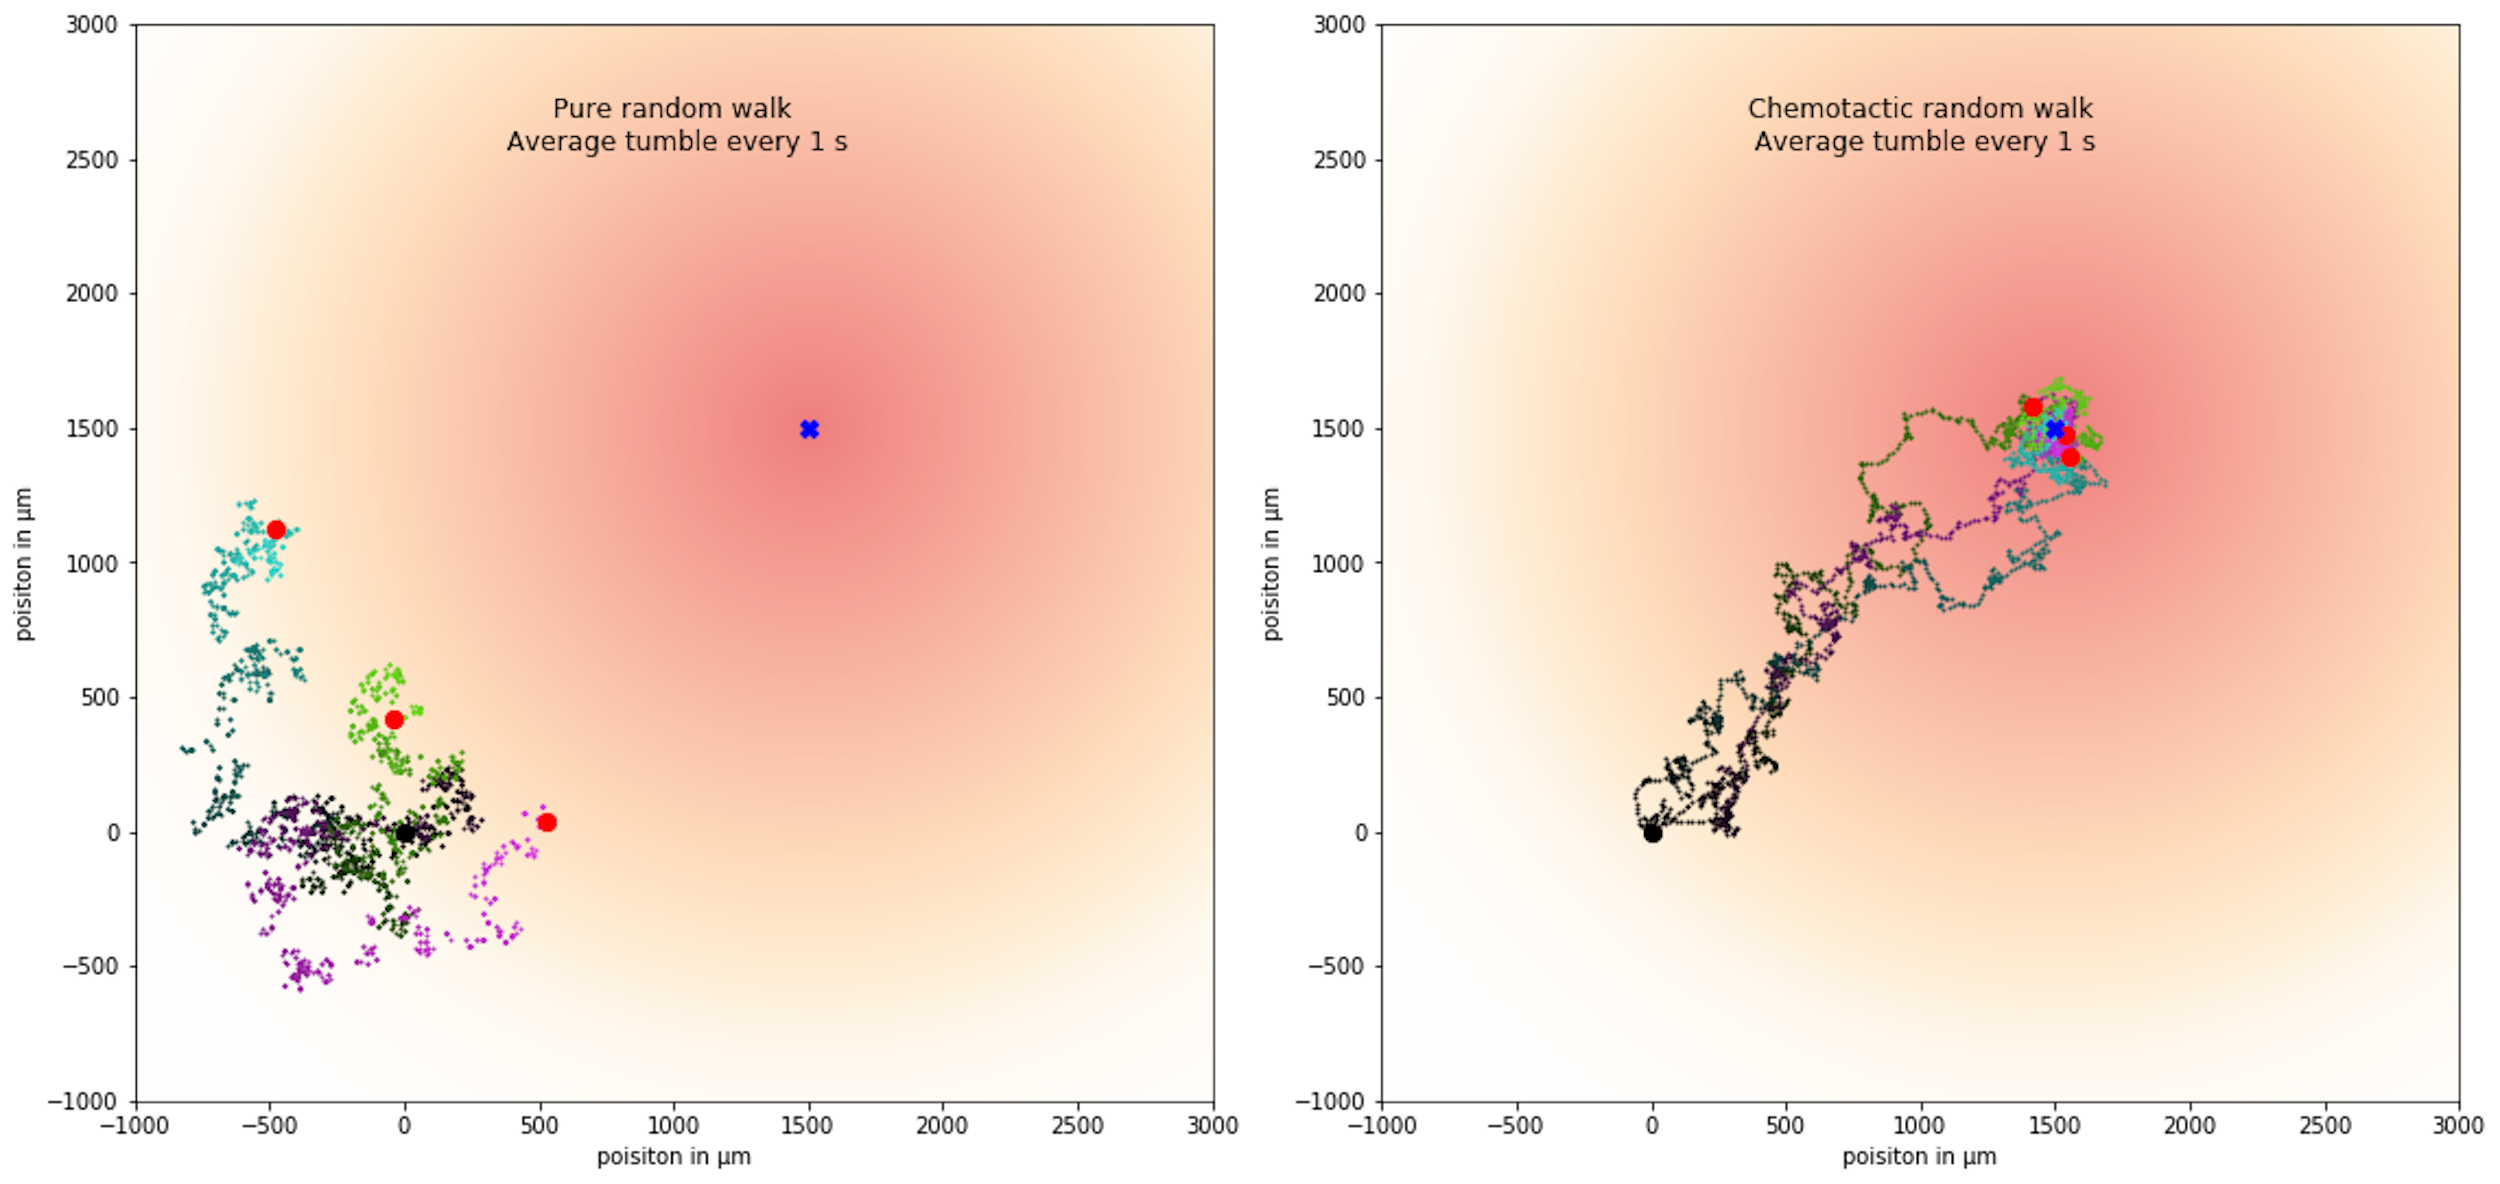
\includegraphics[width = 0.8\textwidth]{../images/chemotaxis_traj_compare_uniform.png}
\caption{Three sample trajectories for each of the two exploration strategies. The standard random walk strategy is shown on the left, and the chemotactic random walk is shown on the right. Regions that are more heavily colored red correspond to higher concentrations of ligand, with a goal having maximum concentration at the point $(\text{1,500}, \text{1,500})$, which is highlighted using a blue square. A single cell's walk is colored from darker to lighter colors across the time frame of the trajectory.}
\label{fig:chemotaxis_traj_compare_uniform}
\end{figure}


Of course, we should be wary of such a small sample size. To confirm that what we observed in these trajectories is true in general, we will compare the two strategies over many simulations. \autoref{fig:chemotaxis_performance_compare_uniform} plots the cell's average final distance to the goal over 500 simulations for both strategies.

\begin{figure}[h]
\centering
\mySfFamily
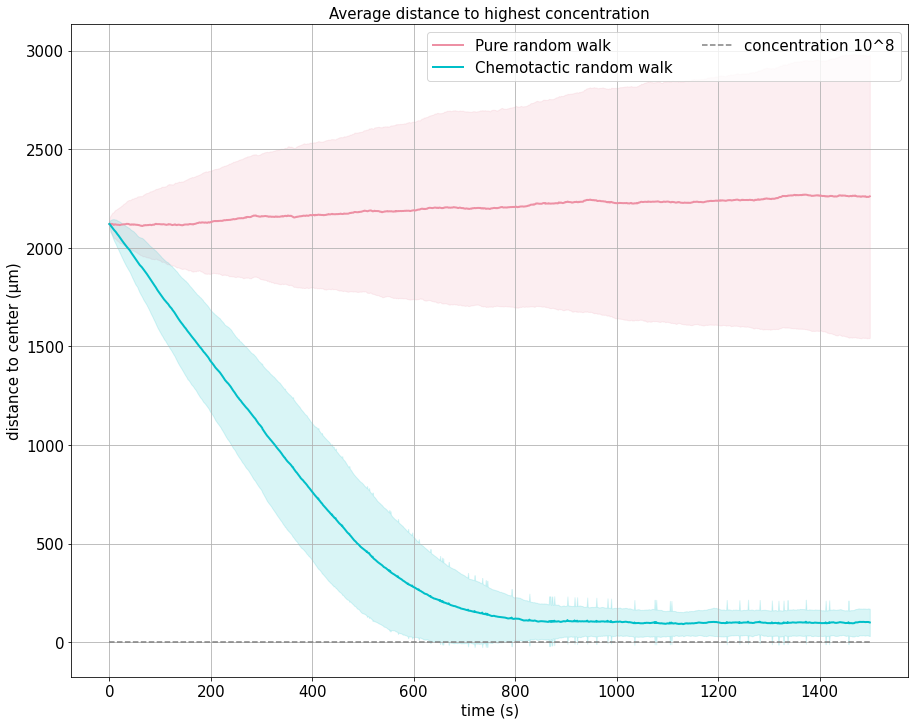
\includegraphics[width = 0.85\textwidth]{../images/chemotaxis_performance_compare_uniform.png}
\caption{Average distance to the goal plotted over time for 500 cellular simulations following each of the two strategies; the standard random walk is shown in red, and the chemotactic random walk is shown in blue. The shaded area around each strategy's plot represents one standard deviation from the average.}
\label{fig:chemotaxis_performance_compare_uniform}
\end{figure}


Using strategy 1, cells have some chance of reaching the goal because they tend to spread out over time, but nothing about this strategy keeps cells at the goal, and so the average distance to the goal does not decrease. In fact, as cells drift away due to random noise, they will on average get farther from the goal. With strategy 2, the cells approach the goal and remain there.

Strategy 2 amounts to a very slight change in strategy 1 in which we allow the cell to run for a greater distance if it senses an increase in the attractant concentration. After all, the direction of travel is still \textit{random}. So why would this strategy be so much better than a pure random walk?

The answer to this quandary is that the attractant detection provides a ``rubber band'' effect. If the bacterium is traveling down an attractant gradient (i.e., away from an attractant), then it is not allowed to travel very far in a single step before it is forced to tumble. If an increase of attractant is detected, however, then the cell can travel farther before tumbling. On average, then, this effect helps to pull the bacterium in the direction of increasing attractant, even though each of its steps is taken in a random direction.

A very small change to a simple, unsuccessful randomized algorithm can produce an elegant approach for exploring an unknown environment. But we left one question unanswered. Why is it that a default tumbling frequency of one tumble per second appears to be stable across a wide range of bacteria?

To address this question, we will see how changing $t_0$, the default time for a run step, affects the ability of a simulated bacterium following strategy 2 to locate the goal. You may like to adjust the value of $t_0$ in the previous tutorial \tutorial[https://biologicalmodeling.org/chemotaxis/tutorial_walk] yourself, or follow the tutorial \tutorial[https://biologicalmodeling.org/chemotaxis/tutorial_tumbling_frequencies].


\FloatBarrier
\phantomsection
\subsection{Why is background tumbling frequency constant across bacterial species?}


The following figures show three trajectories for a few different values of $t_0$ and a simulation that lasts for 800 seconds. First, we set $t_0$ equal to 0.2 seconds and see that the bacteria are not able to walk far enough in a single step to head toward the goal (\autoref{fig:chemotaxis_traj_0.2_uniform}).

\begin{figure}[h]
\centering
\mySfFamily
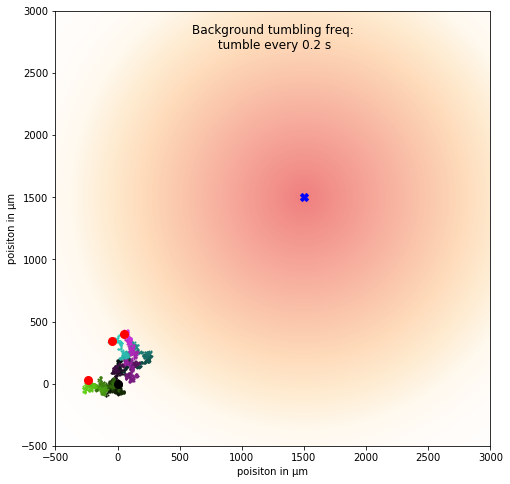
\includegraphics[width = 0.6\textwidth]{../images/chemotaxis_traj_0.2_uniform.png}
\caption{Three sample trajectories of a simulated cell following the chemotactic random walk strategy with an average default tumbling frequency of 0.2 seconds.}
\label{fig:chemotaxis_traj_0.2_uniform}
\end{figure}

If we increase $t_0$ to 5.0 seconds, then cells can run for so long that they may carry on past the goal without being able to apply the brakes by tumbling (\autoref{fig:chemotaxis_traj_5.0_uniform}).

\begin{figure}[h]
\centering
\mySfFamily
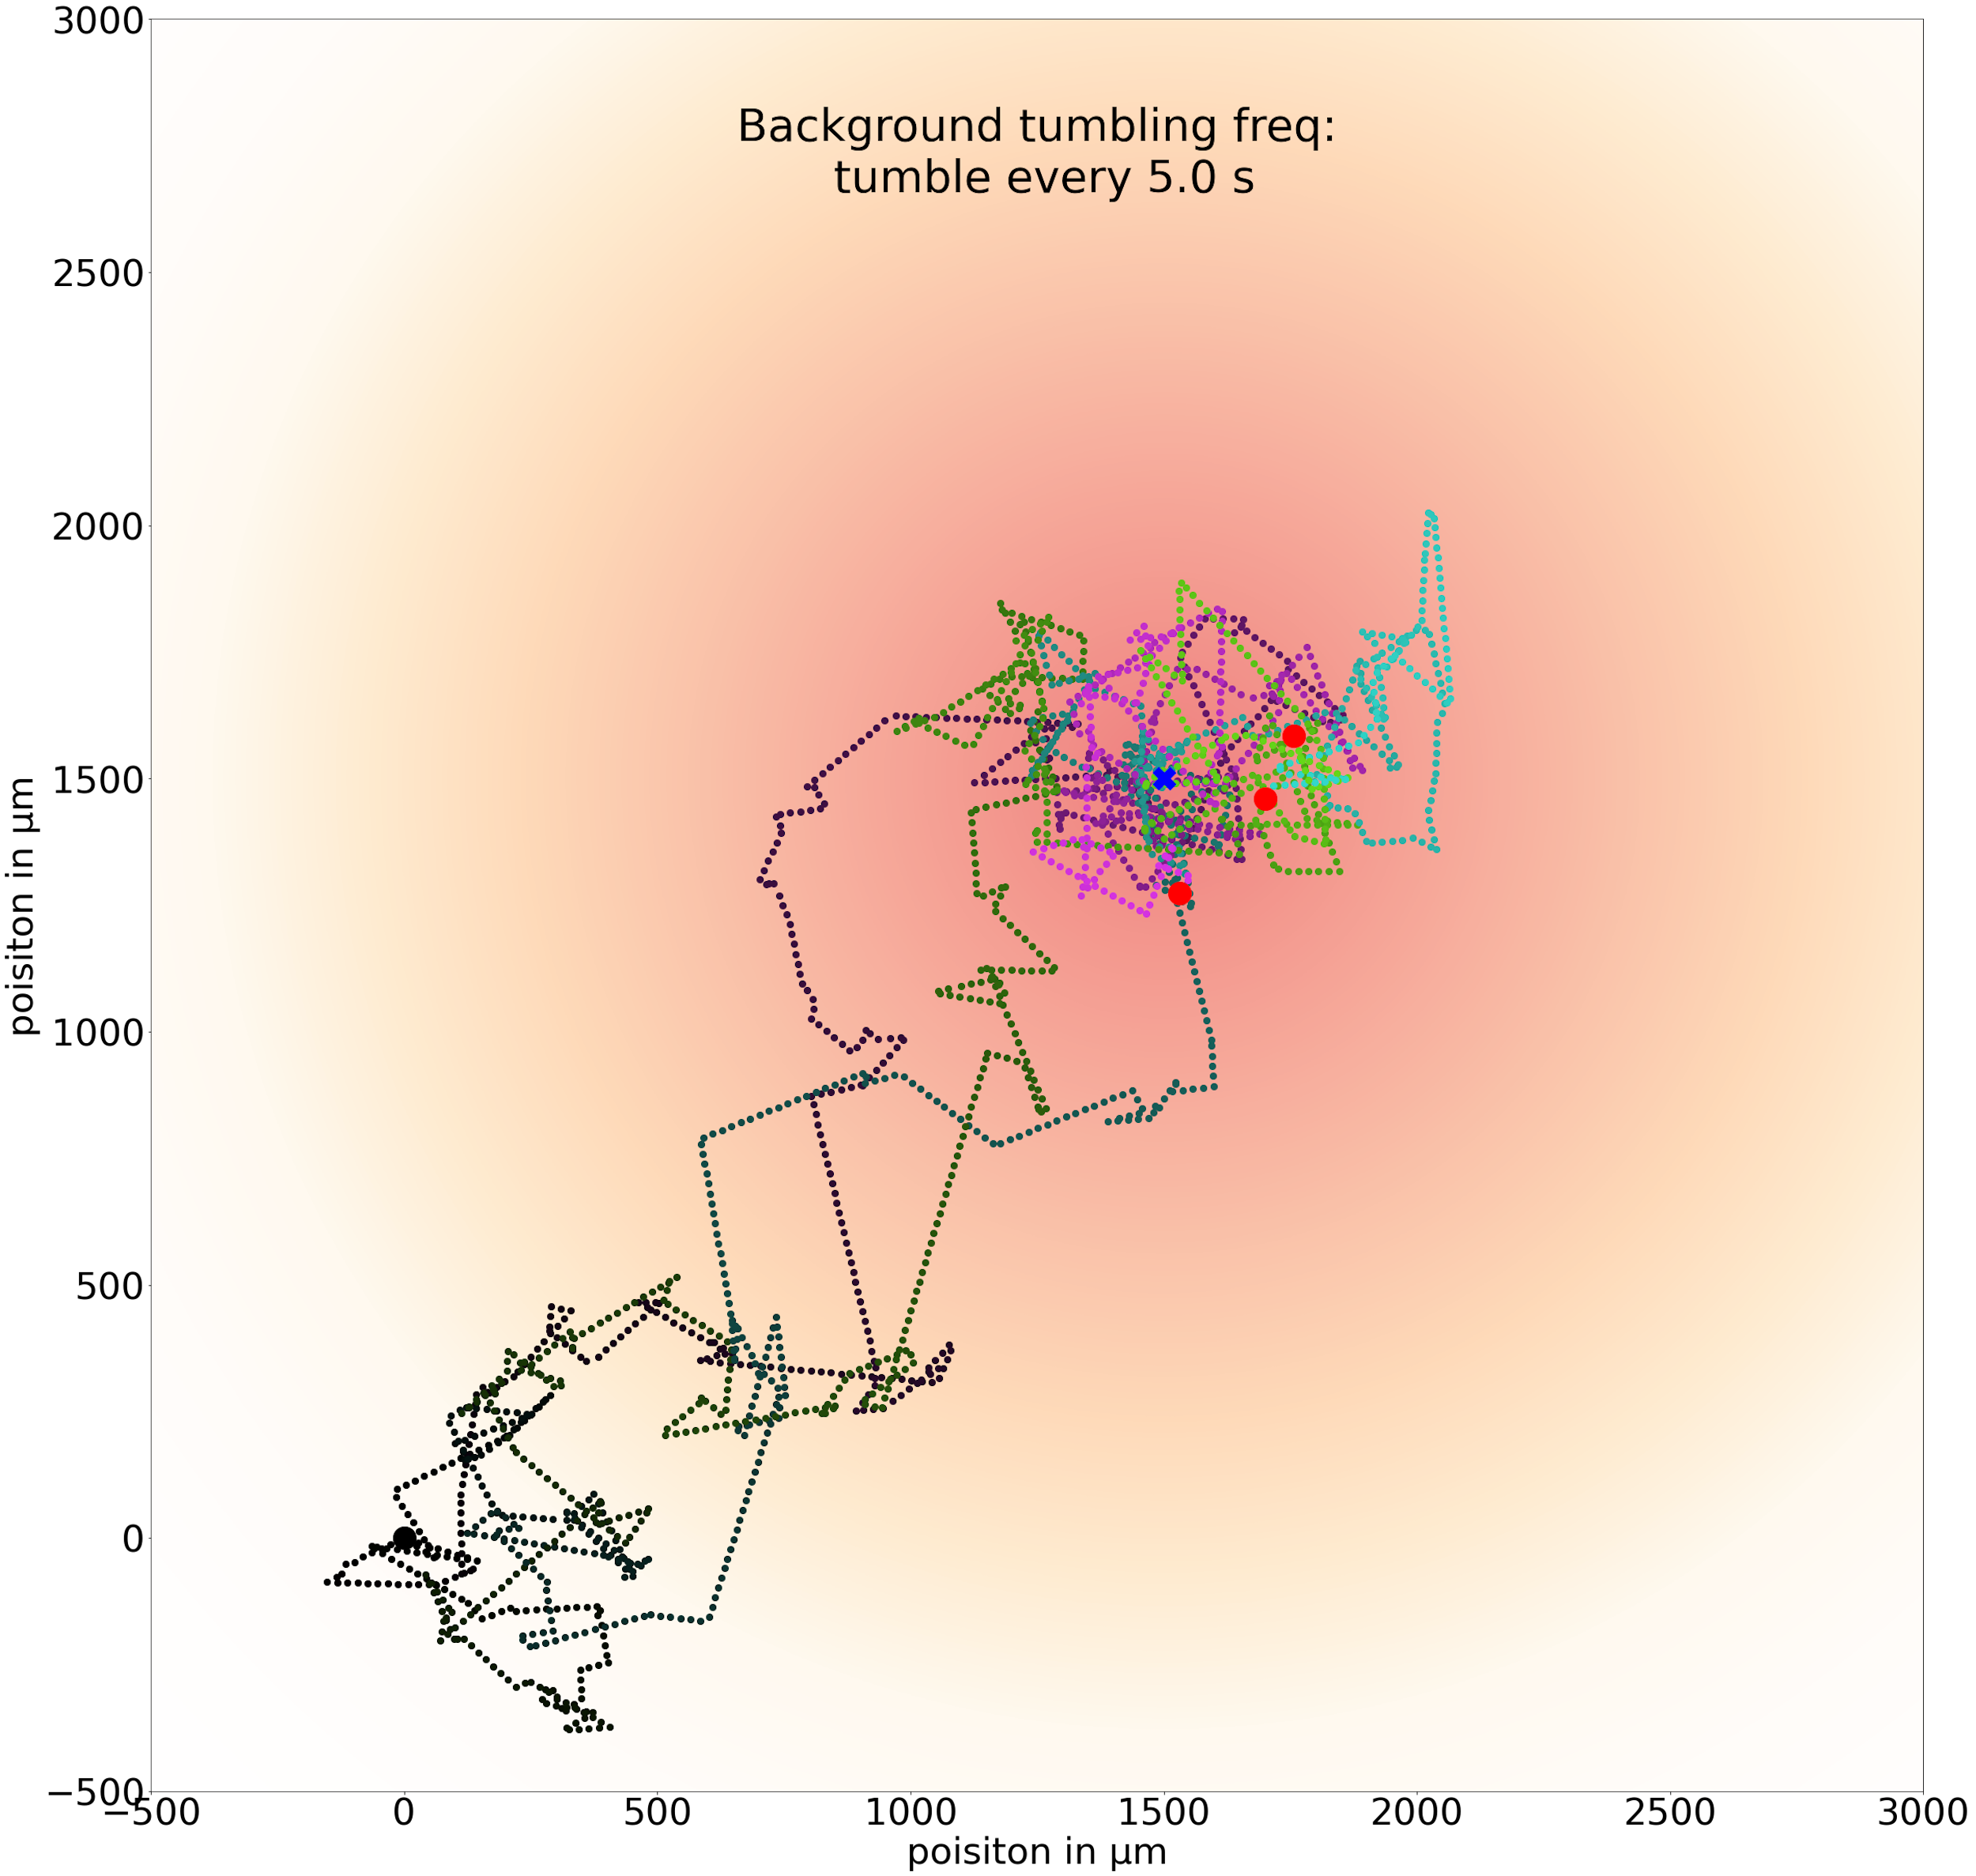
\includegraphics[width = 0.6\textwidth]{../images/chemotaxis_traj_5.0_uniform.png}
\caption{Three sample trajectories of a simulated cell following the chemotactic random walk strategy with an average default tumbling frequency of 5.0 seconds.}
\label{fig:chemotaxis_traj_5.0_uniform}
\end{figure}


When we set $t_0$ equal to 1.0, \autoref{fig:chemotaxis_traj_1.0_uniform} shows a ``Goldilocks'' effect in which the default tumbling time is just right (\autoref{fig:chemotaxis_traj_1.0_uniform}). The simulated bacterium can run for long enough at a time to head quickly toward the goal, and it tumbles frequently enough to keep it there.

\begin{figure}[h]
\centering
\mySfFamily
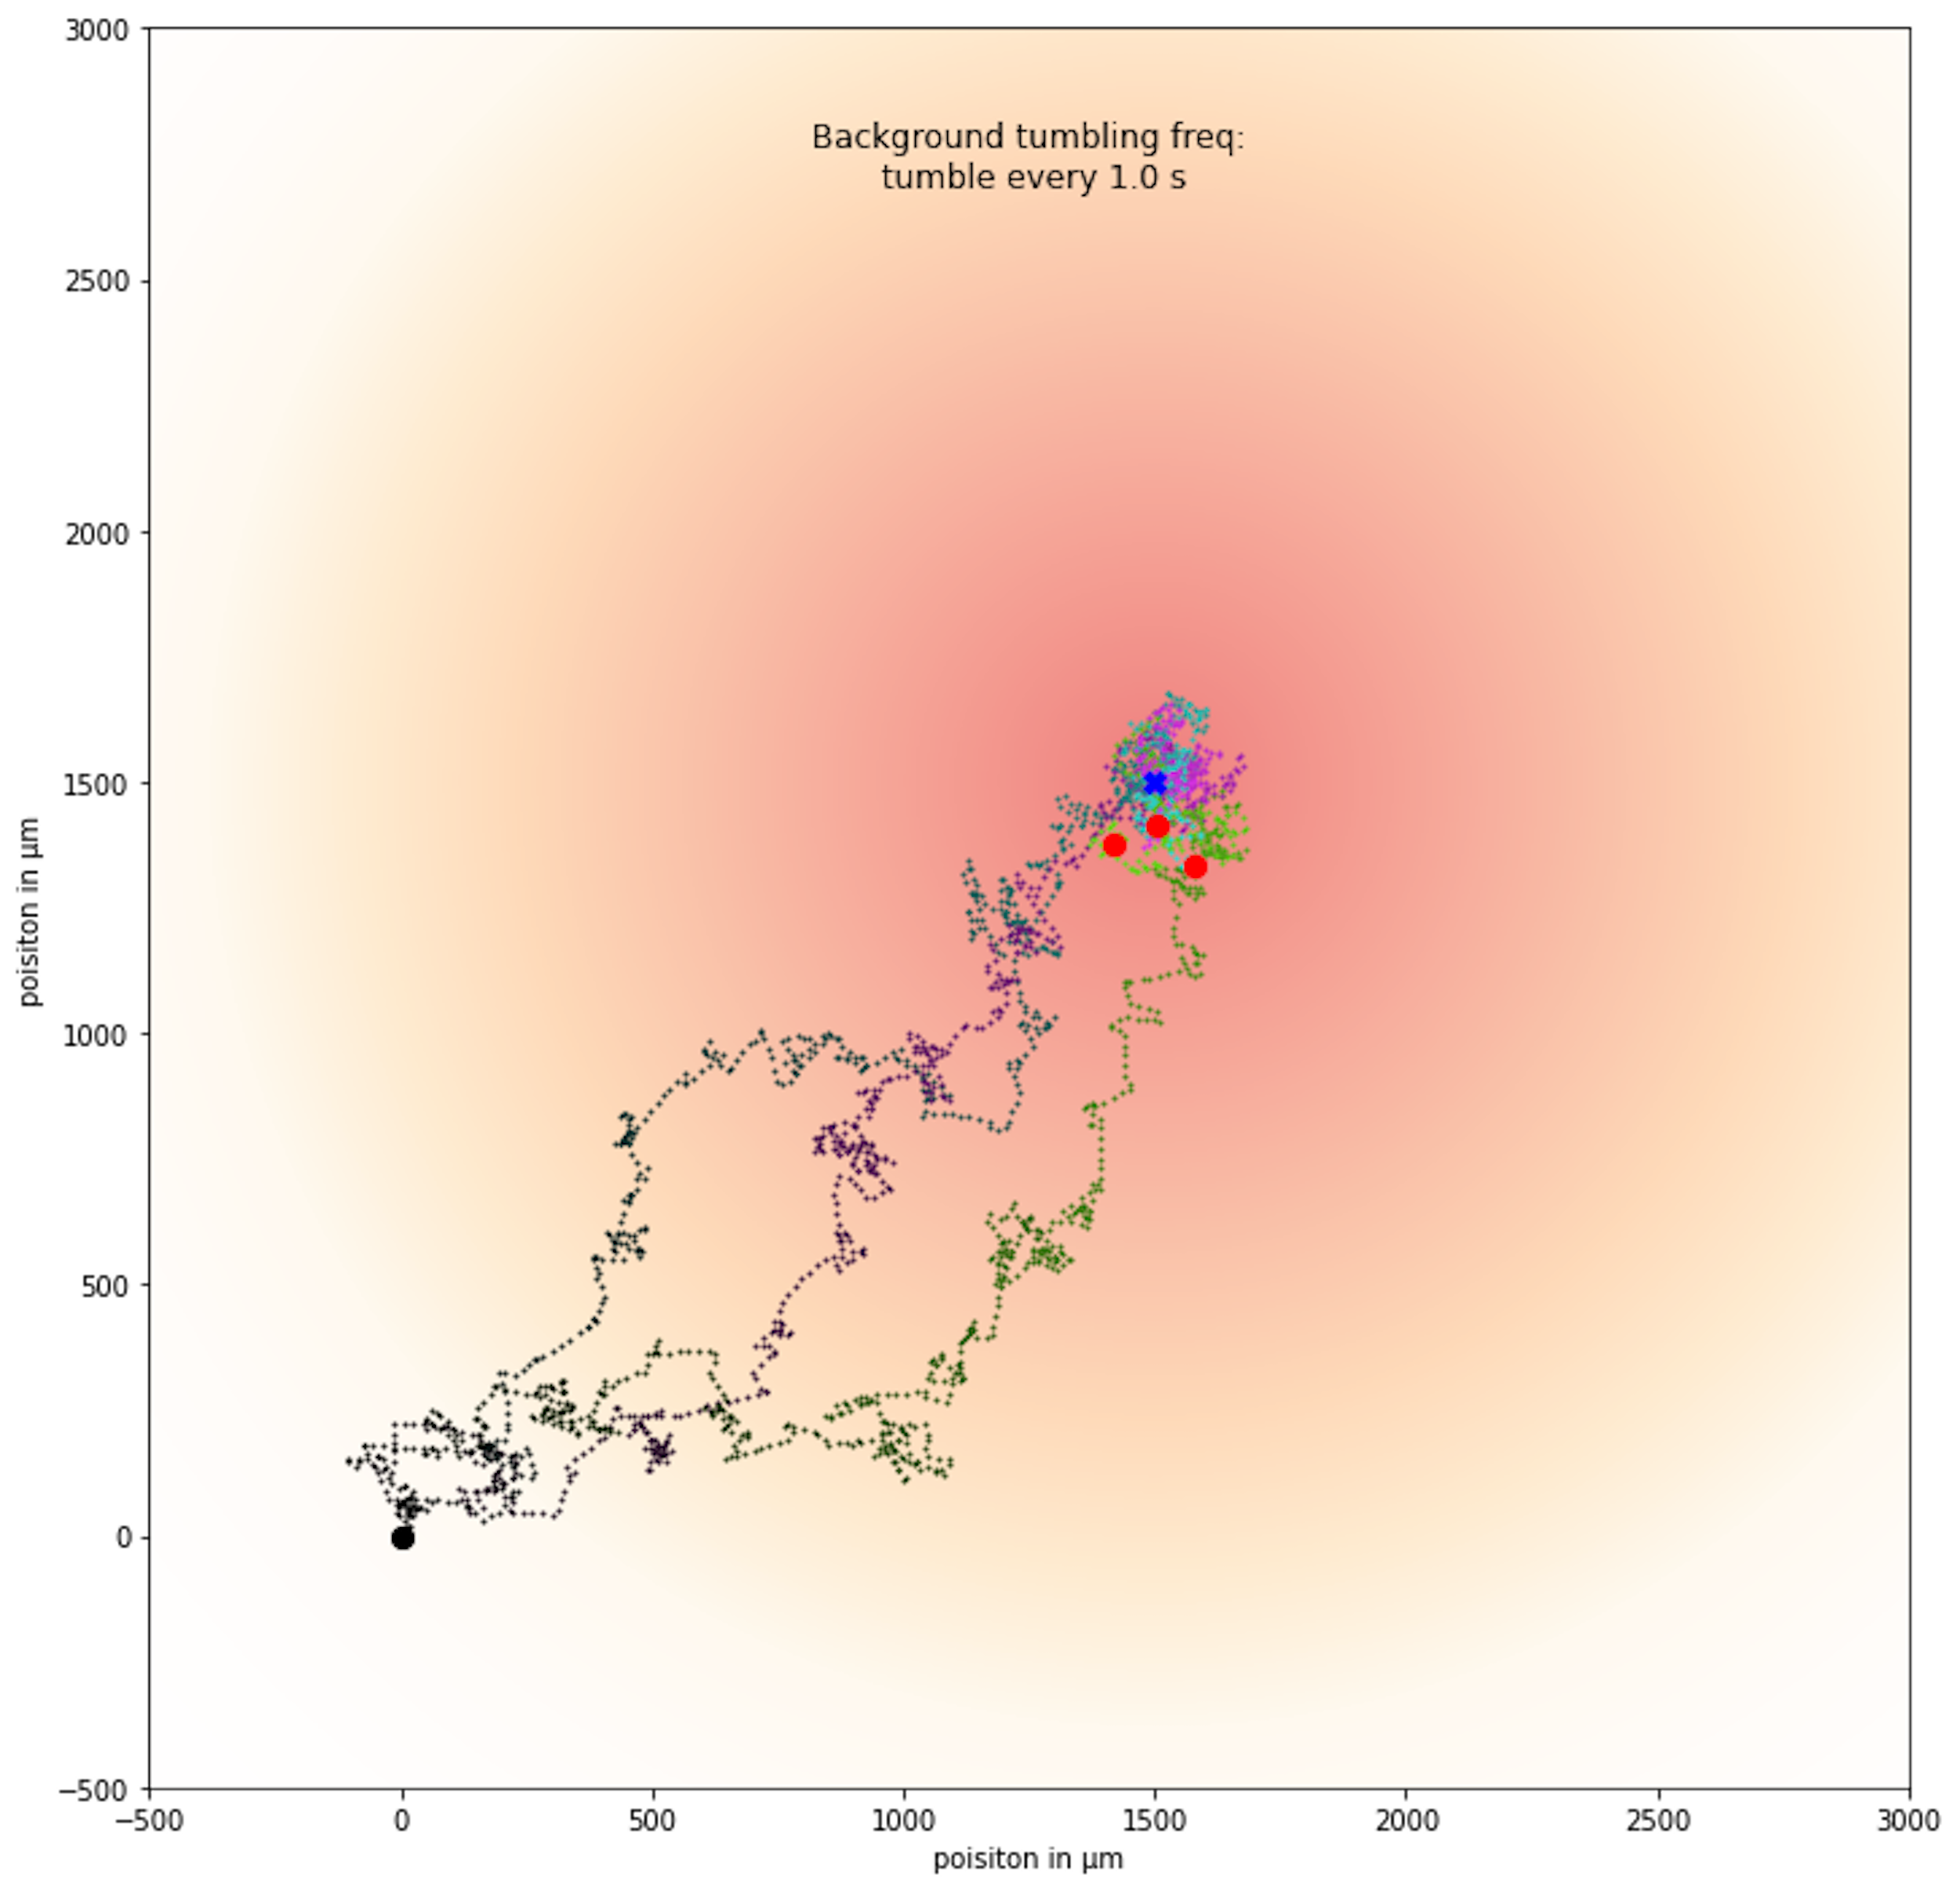
\includegraphics[width = 0.6\textwidth]{../images/chemotaxis_traj_1.0_uniform.png}
\caption{Three sample trajectories of a simulated cell following the chemotactic random walk strategy with an average default tumbling frequency of 1.0 seconds.}
\label{fig:chemotaxis_traj_1.0_uniform}
\end{figure}


\autoref{fig:chemotaxis_performance_uniform} shows a plot of average distance to the goal over time for 500 simulated cells following the chemotactic strategy for a variety of choices of $t_0$, and confirms that a value of $t_0$ approximately equal to one second is ideal for finding an attractant.


\begin{figure}[h]
\centering
\mySfFamily
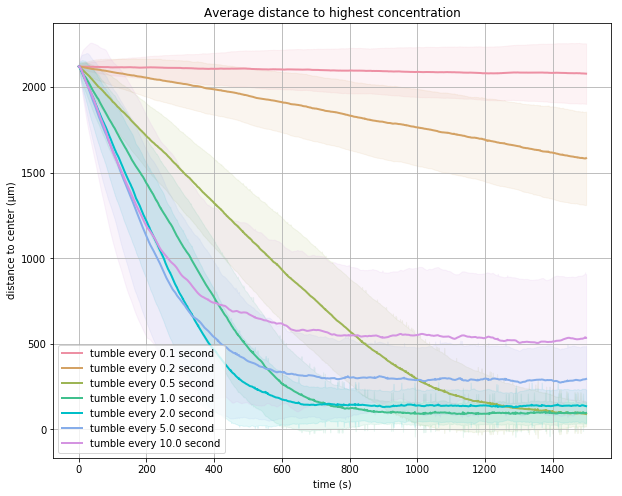
\includegraphics[width = 0.85\textwidth]{../images/chemotaxis_performance_uniform.png}
\caption{Average distance to the goal over time for 500 cells. Each colored line indicates the average distance to the goal over time for a different value of $\textvar{t}_\text{0}$; the shaded area represents one standard deviation.}
\label{fig:chemotaxis_performance_uniform}
\end{figure}

%Below, we reproduce the video from earlier in this chapter showing \textit{E. coli} moving towards a sugar crystal. This video shows that the behavior of real \textit{E. coli} is similar to that of our simulated bacteria. Bacteria generally move towards the crystal and then remain close to it; some bacteria run by the crystal, but they turn around to move toward the crystal again.
%
%\texttt{NEED FIGURE HERE -- TO REPLACE VIDEO}\\

\phantomsection
\subsection{Bacteria are even smarter than we thought}

When we watch bacteria reorient under a microscope, their behavior appears more intelligent than simply walking in a random direction. The reason for this behavior of the bacteria is that like most things in biology, the reality of the system that we are studying turns out to be more complex than we might imagine.

The direction of bacterial reorientation is not completely random, but rather follows a normal distribution with mean of 68° and standard deviation of 36°. That is, the bacterium typically does not tend to make as drastic of a change to its orientation as it would in a pure random walk, which would on average have a change in orientation of 90°.

Yet recent research has shown that the direction of the bacterium's reorientation also depends on whether the cell is traveling in the correct direction. If the bacterium is moving up an attractant gradient, then it makes much smaller changes in its reorientation angle. This allows the cell to stay straight if it is moving in the correct direction but also turn around quickly if it starts heading in the wrong direction. We can even see this behavior in the video above, in which bacteria traveling toward the attractant make only very slight changes in their direction of travel, but reorient themselves more drastically if they overshoot the target.

Bacterial chemotaxis is probably the most studied biological system from the perspective of connecting chemical reactions to the emergent behavior that these reactions cause. Yet for many other systems, this thread connecting a reductionist view of a system to its holistic behavior is still a mystery that will continue inspiring the work of biological modelers for a very long time.


%\FloatBarrier
%\phantomsection
%\section{Citations}
%\citep{Munroe_2014}
%\citep{Pierucci_1978}
%\citep{Sim_2017}
%\citep{Baker_2005}
%\citep{Yong_2016}
%\citep{Weis_1990, Berg_2000}
%\citep{Achouri_2015, Turner_2016, Gotz_1987}
%\citep{Li_2004, Spiro_1997, Stock_1991}
%\citep{Schwartz_2008}
% \citep{Amin_2010, Terwilliger_1986}
% \citep{Spiro_1997}
% \citep{Spiro_1997}
% \citep{Lupas_1989}
%\citep{Boyd_1980}
%\citep{Shimizu_2005, Krembel_2015}
%\citep{Bray_1993}
%\citep{Krembel_2015}.
%\citep{Saragosti_2012}
 
